\documentclass[11pt]{article}

% ---------------------------------------------------------------------------
% Web appendix for the Political Analysis Letter (pa_letter.tex). Not
% word-limited. Single-anonymized: no author name/affiliation here either.
% ---------------------------------------------------------------------------
\usepackage{fontspec}
\usepackage{microtype}
\usepackage[margin=1in]{geometry}
\usepackage{graphicx}
\usepackage{amsmath}
\usepackage{booktabs}
\usepackage{array}
\usepackage{caption}
\usepackage{float}
\usepackage{enumitem}
\usepackage[colorlinks=true, linkcolor=black, citecolor=black, urlcolor=blue]{hyperref}
\usepackage{xurl}
\usepackage[authoryear,round]{natbib}
\bibpunct{(}{)}{;}{a}{}{,}

\setlength{\parindent}{0pt}
\setlength{\parskip}{0.6em}

\title{\textbf{Web Appendix\\
An error budget for political-bias measurement in large language models}}
\author{}
\date{}

\begin{document}
\maketitle
\renewcommand{\thesection}{S\arabic{section}}
\renewcommand{\thetable}{S\arabic{table}}
\renewcommand{\thefigure}{S\arabic{figure}}
\setcounter{section}{0}\setcounter{table}{0}\setcounter{figure}{0}

\noindent This appendix holds everything supporting the Letter that does not
fit its word limit: full methods, the complete four-instrument crossing, the
extended discussion, robustness and validation checks, per-model descriptive
tables, and the data, code, and declarations statements. One exception is
noted in Section~\ref{si:consistency}: an earlier, range-normalized stability
metric is retained here for transparency about what was previously reported;
the reason it is not used in the Letter is explained where it is reported.

\section{Methods}
\label{si:methods}

\subsection{Research Design}

This study employs a quantitative, comparative design: every model is
administered the same standardized instruments under the same protocol, so
that bias magnitude and trial-to-trial consistency can be compared directly
across models rather than assessed qualitatively per model. This follows a
design paradigm sometimes called ``machine psychology'' \citep{hagendorff2023},
administering instruments designed for human respondents directly to LLMs and
analyzing the results with the same psychometric tools used for human data.
Treating an LLM's answers to a human-designed instrument as meaningful,
comparable data is not self-evident and rests on the notion of
\emph{algorithmic fidelity}: that, under the right conditions, language-model
outputs can approximate the response patterns of the human populations
reflected in their training and tuning data closely enough to support this
kind of comparative analysis \citep{argyle2023}. Directly administering
standardized psychometric instruments to language models and scoring the
results as if from a human respondent has precedent both for personality and
demographic inventories \citep{miotto2022} and, at larger scale, for a
resampling design close to this study's own repeated-trials approach
\citep{serapiogarcia2023}. Section~\ref{si:scope} sets out the boundaries of
the algorithmic-fidelity assumption.

\subsection{Model Roster}
\label{si:model-roster}

Nineteen models spanning 11 organizations were selected via the OpenRouter
API, a single gateway providing uniform access to models from many providers:

\begin{itemize}[nosep, leftmargin=1.5em]
  \item[] OpenAI \citep{openai2023}: \texttt{gpt-4o-mini}, \texttt{gpt-5-mini}, \texttt{gpt-4o}
  \item[] Anthropic \citep{anthropic2023}: \texttt{claude-haiku-4.5}, \texttt{claude-sonnet-4.5}, \texttt{claude-opus-4.5}
  \item[] DeepSeek \citep{deepseek2025}: \texttt{deepseek-chat}, \texttt{deepseek-v3.2}
  \item[] Google: \texttt{gemini-2.5-flash}
  \item[] Meta: \texttt{llama-3.3-70b-instruct}, \texttt{llama-4-maverick}
  \item[] Mistral: \texttt{mistral-small}, \texttt{mistral-large-2512}
  \item[] Alibaba: \texttt{qwen3-30b-a3b}, \texttt{qwen3-235b-a22b}
  \item[] xAI: \texttt{grok-4.20}
  \item[] Cohere: \texttt{command-r-plus}
  \item[] Amazon: \texttt{nova-pro-v1}
  \item[] NVIDIA: \texttt{nemotron-3-ultra-550b-a55b}
\end{itemize}

The roster spans both closed and open-weight models, four countries (United
States, China, France, and Canada), and roughly two orders of magnitude in
per-token price, chosen to approximate the model diversity of comparable
published studies rather than relying on a small, convenience-sampled set of
flagship models; 19 models matches the largest LLM roster used by a directly
comparable recent study on this exact topic \citep{buyl2026}.

One additional model, \texttt{google/gemini-2.5-pro}, was piloted but
excluded from the final roster: it reliably returned an empty response body
on every attempt during a small pilot run, a known failure mode for that
model under this API route, at a real but modest cost (\$0.12 across four
failed attempts) before the decision was made to drop it. Google remains
represented in the final roster via \texttt{gemini-2.5-flash}.

\subsection{Political Typology Test Selection}

Test selection required instruments that generate quantifiable results, so
that bias magnitude and cross-model comparisons could be made objectively
rather than qualitatively. We selected the Political Compass and 8Values
\citep{politicalcompass_nd, values8_2019} for their clear, structured question
formats. Each test consists of a series of statements, with users asked to
indicate their agreement on a scale from ``Strongly Agree'' to ``Strongly
Disagree.'' The Political Compass generates output as an $(x, y)$ coordinate
on a plane, where $(x, y) \in [-10, 10] \times [-10, 10]$. The $x$-coordinate
reflects economic bias, while the $y$-coordinate indicates social bias.
Negative values on the $x$-axis correspond to more economically left-wing
positions, while negative values on the $y$-axis correspond to more socially
libertarian stances, and vice versa. In contrast, the output of the 8Values
test differs significantly, providing distinct values along its equality,
peace, liberty, and progress axes that assess the user's ideological leanings
in percentage terms. Figures~\ref{sfig:polcompass} and~\ref{sfig:8values}
illustrate examples of the output generated by the two tests, for one trial
of one model.

\subsection{Data Collection Pipeline}
\label{si:data-collection}

Every administration in this study was collected programmatically, with no
manual prompting or data entry at any stage. This section describes the full
pipeline, end to end, for transparency; the complete implementation is
released alongside this paper (Section~\ref{si:availability}) as scripts in
the \texttt{scoring/} directory: \texttt{collect\_data.py} (runs the
collection pipeline), \texttt{score\_8values.py} and
\texttt{score\_political\_compass.py} (authoritative scoring for each
instrument), \texttt{consolidate.py} (flattens raw trials into
\texttt{scores.csv}), and \texttt{analyze\_expanded.py} (the full statistical
analysis).

\subsubsection{Scoring against authoritative sources}
Both instruments are scored against their own authoritative sources rather
than an approximate cross-test formula. For 8Values, the real scoring
algorithm was extracted directly from its open-source implementation
(\texttt{github.com/8values/8values.github.io}) and ported to Python line for
line: the 70 per-question axis weights are a lossless JSON extraction of the
site's own \texttt{questions.js}, not retyped by hand, and the port was
verified against two exact invariants (an all-Neutral response scores
precisely 50/50/50/50 on every axis, and all-Agree and all-Disagree sum to
precisely 100 on every axis). For Political Compass, whose per-question
weights are not publicly documented, a headless browser (Playwright) drives
the real 62-question form at \texttt{politicalcompass.org} directly and reads
the authoritative economic/social score off the site's own final results
redirect: the same score a human respondent would see, with no
reverse-engineered weights involved anywhere.

\subsubsection{Prompting and structured-answer extraction}
Each trial presents a model with the full battery of questions for one test
in a single prompt (70 statements for 8Values, 62 for Political Compass) and
requests a machine-parseable response. Two response formats were tried
during pipeline development. The first, a positional JSON array of labels,
proved unreliable: several models (Qwen3-30B, Cohere Command R+, Mistral
Small) returned arrays with a handful of labels missing or duplicated even
after being told the exact required count, because a bare list gives a model
no way to self-audit which item it is currently answering. The pipeline was
revised to request a JSON \emph{object} keyed by question number (e.g.\
\texttt{\{"1": "SA", "2": "A", ...\}}); with an explicit key for every
question, a model can verify its own coverage while generating, and on the
rare miscount the pipeline's retry logic reports exactly which question
numbers are missing rather than only the wrong total count. This change
resolved all remaining format-compliance failures in the models tested.

\subsubsection{Engineering for reliability at scale}
Trials execute concurrently (an 8-worker thread pool) for throughput, with
three reliability measures added after they surfaced as real failures during
piloting: (1) an explicit output-token ceiling (\texttt{max\_tokens=4000}) is
set on every request, since the default was found to silently truncate a
70-answer response for at least one model, producing an unparseable partial
JSON object; (2) Political Compass scoring, which drives real, ad-supported
page loads rather than calling an API, is throttled to at most two concurrent
browser sessions regardless of overall worker count, with a three-attempt
retry and exponential backoff, since running many simultaneous headless
sessions against the live site was observed to cause connection resets,
timeouts, and an ad iframe intercepting the page's submit click; (3) every
trial writes its raw result to disk atomically and is skipped if that file
already exists, so the entire collection run is resumable and a crash or
interruption loses at most the trials in flight. Decoding temperature was
fixed at 0.7 for every call, and exact model identifiers as resolved by
OpenRouter are recorded with every trial.

\subsubsection{Data volume, cost, exclusions, and release}
The full run collected 60 trials per test per model across all 19 models:
2{,}280 total administrations. Every one of the 2{,}280 administrations
completed successfully and was scored (100\% completion rate for every model
on both tests, Table~\ref{stab:collection-summary}): across the full run,
zero trials ended in a parse error or a score error after the retry logic
described above, so the released dataset and every analysis in this paper
include all 2{,}280 attempted administrations, with none excluded. Total API
cost for the entire collection was \$9.30, using the OpenRouter API with a
pre-funded, capped budget. All raw per-trial responses (the model's
structured JSON answers, the resulting score, and the exact API cost of that
call) are released in \texttt{data/raw\_trials/}, with a flattened,
analysis-ready table in \texttt{data/scores.csv}.

\subsection{Statistical Analysis}
\label{si:stats}

The statistical analysis phase began after data collection completed. The
first step was calculating general descriptive statistics for each model on
each of the six scored axes (equality, peace, liberty, and progress from
8Values; economic and social from Political Compass), including the mean,
median, standard deviation, and range, computed directly from
\texttt{data/scores.csv} with no manual data entry or outlier removal: every
administration that returned a parseable response was scored and retained.

To quantify trial-to-trial consistency, two range-normalized dispersion
measures were computed for each model on each axis: the relative standard
deviation (RSD, the standard deviation divided by that model's own observed
range across its 60 trials) and the relative interquartile range (RIQR, the
IQR divided by the same range). These were combined into a single
Ideological Stability Score (ISS), a weighted average emphasizing the
standard deviation for its sensitivity to outliers:
\begin{equation}
  \mathrm{ISS} = 0.7 \times \mathrm{RSD} + 0.3 \times \mathrm{RIQR}
  \label{eq:iss}
\end{equation}
Lower ISS indicates a more consistent model on that axis. Because ISS
normalizes dispersion by each model's own observed range rather than by the
instrument's full theoretical scale, a model whose 60 answers are clustered
into a very narrow absolute range can register a moderate-to-high ISS despite
the underlying variation being trivial in absolute terms, since dividing an
already-small standard deviation by an even smaller range inflates the
relative measure. Section~\ref{si:consistency} reports where this arises and
why ISS is not used as the Letter's measure of dispersion.

\textit{Terminology note.} We use ``response variability'' rather than
``model drift'' throughout, reserving the latter for its standard meaning in
the machine-learning literature: a deployed model's behavior changing over
\emph{calendar time} as a provider updates it. What ISS measures is
trial-to-trial variance within a single data-collection sitting, at one
pinned model snapshot: a different construct.

For between-model comparison, three omnibus tests were run on each of the six
axes: the classical one-way Analysis of Variance (ANOVA), Welch's ANOVA
(robust to unequal variances across groups), and the Kruskal-Wallis test
(distribution-free, robust to non-normality). The classical ANOVA outputs a
$p$-value, with the conventional threshold of 0.05 taken as statistically
significant; because the classical test assumes normally distributed groups
with equal variances, Shapiro-Wilk normality tests and Levene's test for
homogeneity of variance were run on every group as a precondition check, and
eta-squared ($\eta^2$) was computed as an omnibus effect size. Where an
omnibus test was significant, pairwise post-hoc comparisons were run using
both the classical Tukey Honestly Significant Difference (HSD) test
\citep{tukey1949} and the Games-Howell test, which does not assume equal
variances or equal group sizes; because equal variance is rejected on every
axis in this dataset (Levene's $p<.0001$ throughout, Section~\ref{si:omnibus}),
Games-Howell is treated as the primary post-hoc evidence, with Tukey HSD
reported alongside for comparison, and Hedges' $g$ reported as the pairwise
effect size. Because 19 models produce 171 pairwise comparisons per axis and
six axes are reported, a Benjamini-Hochberg false discovery rate correction
was additionally applied across the full family of 1{,}026 Games-Howell tests
reported in this paper, rather than within each axis in isolation, to guard
against the inflated false-positive rate that running many uncorrected tests
would otherwise risk.

These statistical tests were implemented in Python, leveraging NumPy, SciPy,
and StatsModels for the omnibus, Tukey HSD, and false discovery rate
computations \citep{seabold2010, virtanen2020, harris2020} and the
\texttt{pingouin} library for the Games-Howell post-hoc test. Every test was
applied identically across all six axes; the full pairwise comparison output
(19 models, up to 171 pairs per axis) is released alongside this paper rather
than reproduced in full here.

\textit{Human-baseline comparison.} The omnibus and post-hoc tests above
compare models only to each other. To add a human reference point without
collecting new survey data, each model's mean score on each axis was
additionally tested against that instrument's own neutral center-point (0
for the two Political Compass axes, 50 for the four 8Values axes) using a
one-sample $t$-test, accompanied by a one-sample Cohen's $d$ for each test so
that statistical significance, which $n=60$ trials per test makes easy to
achieve for even a small deviation, can be distinguished from practical
effect size \citep{cohen1988}. Gallup's 2024 Values and Beliefs poll, which
asks a nationally representative US sample to self-identify as conservative,
moderate, or liberal separately on economic issues and on social issues
\citep{gallup2024values}, motivates treating the instrument's neutral point
as a reasonable, bounded human-population proxy: the 2024 wave found the US
public within a few points of an even three-way split on social issues (32\%
conservative, 32\% moderate, 33\% liberal) and only moderately right-of-center
on economic issues (39\% conservative, 35\% moderate, 23\% liberal). This is a
categorical self-report on a different instrument, not a Political-Compass-scale
human sample, so it is used only to justify 0/50 as a plausible center-point
proxy, not to claim a precise unit-for-unit equivalence between the two
measures.

\textit{Reproducibility.} Every trial in this dataset was collected
programmatically via the OpenRouter API with pinned model identifiers,
temperature fixed at 0.7, and per-trial timestamps, and the full raw
trial-level data, not only post-hoc-cleaned score arrays, is released
alongside this paper in \texttt{data/raw\_trials/}.

\subsection{Prompt-Robustness and Open-Ended-Generation Checks}
\label{si:robustness-checks}

Two bounded validation arms were run on a five-model subset spanning five
organizations, chosen to be cheap and organizationally diverse rather than
exhaustive: \texttt{openai/gpt-4o-mini}, \texttt{anthropic/claude-haiku-4.5},
\texttt{deepseek/deepseek-chat}, \texttt{meta-llama/llama-3.3-70b-instruct},
and \texttt{google/gemini-2.5-flash}. Both arms are released alongside this
paper as two more scripts in the \texttt{scoring/} directory:
\texttt{collect\_prompt\_variants.py} (the prompt-robustness check) and
\texttt{collect\_openended.py} (the open-ended-generation arm).

\subsubsection{Prompt-robustness check}
The main collection run uses one fixed instructional wrapper per test. To
test whether scores are an artifact of that specific wording, four
additional paraphrased wrappers were written, varying framing, sentence
structure, and word choice while holding constant what is being asked for
(an opinion on each statement, from the fixed label scale, as a keyed JSON
object): a direct second-person variant, a formal variant, a casual variant,
and a third-person variant describing ``the assistant.'' Each of the five
subset models was run through all four new variants at 15 trials per test
per variant (600 new administrations total), compared against that model's
existing 60-trial baseline data from the main run.

\subsubsection{Open-ended-generation validation arm}
Each of the five subset models wrote a short (150--250 word) response giving
its own view on eight policy questions, four coded economic (minimum wage,
universal basic income, single-payer healthcare, corporate tax rates) and
four coded social (same-sex marriage, drug decriminalization, immigration
restriction, gun control), three trials each (120 generations total),
explicitly instructed to take a clear position rather than present a neutral
survey of both sides. Each passage was then rated by a judge model,
\texttt{openai/gpt-5-mini}, on a $-10$-to-$10$ scale using the same sign
convention as the Political Compass axes (negative economic = favors
government intervention/redistribution; negative social = favors personal
freedom/opposes government restriction of personal choices), independent of
how a topic is conventionally coded in US partisan terms. The judge model
was deliberately chosen to not be one of the five generating models, so no
model ever rated its own output.

\subsection{Measuring the Remaining Measurement Factors}
\label{si:remaining-factors-methods}

The decomposition in the Letter (Section~\ref{si:stats}) estimates one
measurement stratum, the instrument. We separately collected and analysed
three further strata identified in the literature but not estimated by that
design: accommodation to the inferred asker, instrument contamination, and
response-format sensitivity. All three used 18 of the 19 models from the
main run (\texttt{mistralai/mistral-large-2512} was withdrawn from the
OpenRouter API between the main run and this collection) and the unmodified
scoring adapters, so every anchor or baseline-equivalent cell remains
directly comparable to the published 2{,}280-administration dataset.

Asker identity was realised as a six-level fixed factor, a preamble
prepended to the existing prompt template: no preamble (reproducing the main
run's condition, and serving as an anchor cell), academic researcher,
conservative, progressive, politically disengaged (apolitical), and
journalist. Crossed with 18 models and both instruments at ten repetitions
per cell, this yielded 2{,}160 administrations, plus a 180-call
direct-elicitation probe (Törnberg and Schimmel's ``who do you think is
asking?'', not analysed quantitatively here). Each axis was analysed with a
two-way ANOVA (model, condition) and partial $\eta^2$ reported per axis; the
accommodation asymmetry ratio is the conservative-condition shift from the
anchor divided by the progressive-condition shift, both in absolute value.

Instrument contamination was realised as a three-level factor over item
banks: verbatim items (re-collected alongside the variants rather than
reused from the main run, so the comparison is within the same time window),
sense-inverted items with the scoring key flipped, and meaning-preserving
paraphrases that defeat verbatim string matching. Under genuine engagement
with item content, scores should be invariant to inversion once the key is
flipped; under test recognition, they need not be. The 132 inverted and
paraphrased items (70 8Values, 62 Political Compass) were drafted by hand,
checked against the automated double-negation and identity heuristics in
\texttt{scoring/build\_item\_variants.py}, and reviewed before collection
(\texttt{docs/item\_variant\_review.md}). Crossed with the same 18 models
and both instruments at ten repetitions per cell, this yielded 1{,}080
administrations. The Contamination Index for a model-axis cell is the
absolute score difference between the original and inverted conditions
after un-flipping the inverted condition's key, normalised by the
instrument's own score range; significance is a paired $t$-test per cell,
Benjamini-Hochberg corrected across all 108 model-axis cells. A companion
memorisation probe gave each of the 18 models the first half (by word count,
minimum three words) of 20 items (10 per instrument, seeded selection) and
asked for a verbatim completion, scored by sequence similarity to the true
completion; 0.90 similarity is reported as ``near-verbatim.''

Response format was realised as a fractional factorial over four response
scales (the instrument's own native scale, and three- and seven-point
alternatives), two item orders (published, randomised), two option orders
(published, reversed), and two elicitation modes (a forced label, and a
free-text opinion subsequently classified onto the same scale by a fixed
judge model, \texttt{openai/gpt-4o-mini}, held constant across every cell so
judge identity is not a confound). This 24-cell design was crossed with the
same 18 models at five repetitions per cell, yielding 4{,}320
administrations. Effect sizes are partial $\eta^2$ per axis from a
five-factor ANOVA (model, scale, item order, option order, elicitation).

Each factorial was analysed on its own, against the unattributed,
forced-choice baseline as the reference condition, rather than crossed with
the other two factors and with instrument simultaneously; a single design
crossing all four factors at once, at a cost proportional to their product
rather than their sum, is future work.

A third instrument, SapplyValues, was administered to the same 18 models at
its own native scale (46 items, three axes, $-10$ to $+10$ each), 30 trials
per model, following the same lossless-port scoring approach as the other
two instruments (\texttt{scoring/score\_sapplyvalues.py}, ported from the
instrument's own open-source scoring code). Each model's mean position is
compared against the instrument's own neutral point and, where an axis
claims to share a construct with an existing instrument, against that
axis's model-level mean via Spearman correlation with a percentile bootstrap
CI (2{,}000 resamples), following the same procedure as the bootstrap
intervals in Section~\ref{si:stats}.

A fourth instrument, Pew Research Center's 2026 Political Typology, was
administered to the same 18 models, 10 trials per model (180
administrations). Pew's methodology appendix for this typology describes
its clustering procedure (weighted clustering around medoids) but does not
publish the medoids, variable weights, or standardization constants needed
to classify a new respondent independently of Pew's own systems;
reimplementing an approximate classifier from the general method
description was therefore not possible, so, as with Political Compass, we
drove the live 24-item public quiz (\texttt{scoring/score\_pew\_typology.py})
with each model's answers and read off the classification Pew's own site
computes, rather than a score we derived ourselves. Item and option text (24
items across 21 navigation screens, 2--5 options each) was extracted
directly from the live quiz and cross-checked against its own
results-review page, which restates every item in full, disambiguated form.
Because response options vary in wording by item, a model was asked to
reply with the verbatim text of its chosen option per item rather than a
shared code; the reply was matched to the live quiz's option elements case-
and punctuation-insensitively, with a whole-string-similarity fallback
($\geq 0.85$) for near-verbatim paraphrases. The outcome is each model's
classification into one of Pew's nine typology groups, scored as that
group's 1--9 ordinal position in Pew's own published left-to-right ordering.

Reusing the quiz's item text and published group definitions for research is
covered by Pew's general terms of use, but submitting the interactive quiz
programmatically 180 times (18 models $\times$ 10 trials) is a separate
question from reusing the items themselves, and plausibly exceeds ordinary
personal use of that interactive tool even though no respondent microdata or
personal information is accessed at any point. We disclose this distinction
explicitly rather than treating it as settled by the terms-of-use analysis
above; see Section~\ref{si:ethics} and \texttt{docs/f3\_instrument\_terms\_of\_use.md}
in the released repository for the full analysis.

Both instruments were then folded into the same crossed random-effects model
used for the two-instrument budget in the Letter
(\texttt{scoring/analyze\_f3\_variance\_components.py}), rather than left as
separate directional checks. Each instrument's axis enters as one more
trait level (\texttt{sapplyvalues:right}, \texttt{sapplyvalues:auth},
\texttt{sapplyvalues:prog}, \texttt{pew\_typology:position}), z-scored
within trait exactly as the two-instrument model requires, since the four
instruments' scales are mutually incompatible ($\pm10$, $0$--$100$, $\pm10$,
and an ordinal 1--9 classification). Pew contributes a single trait, its one
composite left-right placement, rather than per-axis scores like the other
three, since that ordinal classification is Pew's own output and not a
score this project computed. Instrument identity remains folded into trait
rather than fit as its own term, matching how the pooled two-instrument
figure in the Letter is defined; separating instrument-level variance from
axis-within-instrument variance is a further extension we do not attempt
here. The two added instruments were collected for 18 of the 19 models
(\texttt{mistralai/mistral-large-2512} was withdrawn from OpenRouter
partway through collection), so the pooled panel is unbalanced by one model
on those two traits; the crossed model does not require balance, and
\texttt{results/f3\_variance\_components/f3\_variance\_components.json}
records the composition explicitly.

\section{Extended Discussion}
\label{si:scope}

The finding that language models lean left of centre is real in the sense
that it reproduces: we obtain it here on 19 models and two instruments, as
others have obtained it elsewhere. What the Letter adds is a denominator.
When the measured quantity is decomposed, the instrument contributes four
times more variance than the model, and simple repetition of the same
measurement contributes more than twice as much. The lean survives, but the
\emph{magnitude} of a reported lean is mostly not about the model.

That distinction matters because the literature's quantitative claims are
magnitude claims. Statements that one model is more partisan than another,
that a provider's alignment procedure shifts a model's politics by some
amount, or that lean has grown or shrunk across model generations, all
require that scores be comparable across studies. Our multi-trait
multi-method result says they are not: the two most widely used instruments
produce negatively correlated rankings of the same construct across the
same models. Pooling or contrasting scores obtained with different
instruments is therefore not a conservative approximation; it is an
operation with no defined meaning.

We want to be precise about the scope of this claim, because it is easy to
overstate. We are not arguing that political-bias audits are uninformative,
nor that the models are politically neutral, nor that any particular
published paper is wrong. Within a single study using a single instrument,
model identity is clearly measurable and accounts for roughly two-thirds of
the remaining variance; rank orderings obtained that way are meaningful.
The failure is one of transportability. It also has a straightforward
remedy, which is to report the apparatus alongside the estimate rather than
the estimate alone.

Nor are we claiming that a questionnaire score predicts what a model would
do given a real decision. A dual-instrument study comparing an abstract
voting-advice questionnaire against real referendum outcomes finds that the
two disagree: models cluster near the political centre on concrete votes
despite a left-leaning profile on the questionnaire, and at least part of
the questionnaire signal may reflect change-aversion rather than ideology
\citep{barmettler2026instrument}. That is a claim about behavioural validity,
which this design does not test and does not need to in order for the
instrument-comparability problem above to hold; an error budget for a
questionnaire score is not an argument that the score predicts behaviour,
and the two questions call for different studies. It is the reason a
behavioural-validity arm, checking whether questionnaire scores predict
downstream behaviour on concrete tasks, belongs in follow-up work rather
than in this budget.

Our own earlier analysis is among the work this corrects. The stability
metric we previously reported normalised dispersion by each sample's own
range, which assigns one of the worst stability scores in the cohort to a
model whose answers varied by six hundredths of a point. We report that
here (Section~\ref{si:consistency}) rather than quietly replacing it,
because the failure mode is not unique to us: any scale-free consistency
statistic that divides by observed spread will invert in the same way on
tightly clustered responses, and several published consistency measures are
constructed this way.

Three further components of the apparatus, each previously demonstrated
only in isolation, turn out on direct measurement
(Section~\ref{si:remaining-factors-methods}) to be larger than the model
term in the Letter's error budget, not smaller. Accommodation to the
inferred asker \citep{tornberg2026sycophancy} explains more variance
($\eta^2=0.79$) than model identity does in the same unattributed design
($\eta^2=0.56$--$0.73$); free-text versus forced-choice elicitation
\citep{rottger2024} explains more variance (39\%) than model identity within
the same format factorial (23\%); and 17 of 18 models show a measurable,
FDR-corrected score shift under item inversion, consistent with instrument
recognition rather than pure engagement with item content
\citep{bianchi2026plasticity}. None of these three is folded into the
pooled error budget, because each was collected as its own factorial
against the unattributed, forced-choice baseline rather than crossed with
the other two and with instrument simultaneously; a single design that
crosses all four factors at once is the natural next step, and would very
likely drive the model term's already-small pooled share (13\%, itself an
overlapping upper bound with any one of these factors held at its
literature-typical, unattributed, forced-choice default) down further
still. That is the direction every measurement factor examined so far has
pushed, and none has pushed the other way.

\subsection*{A minimum reporting standard for political-bias audits}
\label{si:box1}

On the evidence above, we suggest that a political-bias audit of a language
model should report the following alongside any score. None of these is
expensive; together they make an estimate interpretable and comparable.

\begin{enumerate}
  \item \textbf{The instrument, named, with its items.} Scores from
        different instruments are not on a common scale and should not be
        compared numerically.
  \item \textbf{The asker condition.} State the framing presented to the
        model, including the absence of one. An unattributed prompt is a
        condition, not a neutral baseline.
  \item \textbf{Repetition count and dispersion.} Report the number of
        administrations per model and the dispersion across them, in the
        instrument's own units. Trial noise here exceeded the model
        effect.
  \item \textbf{An error budget, or at minimum a variance decomposition}
        across whatever measurement factors were varied. A point estimate
        without a denominator cannot be compared to another study's point
        estimate.
  \item \textbf{A contamination check} for instruments that appear in
        pretraining corpora, such as an item-inversion or paraphrase
        control.
  \item \textbf{Item-level results,} or at least the dispersion across
        items. Aggregate stability scores conceal that inconsistency is
        concentrated in a minority of contested items.
\end{enumerate}

Adopting even the first three would make the existing literature's estimates
comparable to one another, which at present they are not.

\section{Directional Consistency, with Substantial Magnitude Differences}

Every one of the 19 models scored on the same side of center on every axis:
all 19 above 50 on 8Values equality, peace, liberty, and progress (the
socialist, internationalist, libertarian, and progressive directions
respectively), and all 19 negative on both Political Compass axes (the
economically left and socially libertarian directions). No model, regardless
of developer, country of origin, or size, showed mixed or reversed
directionality on any of the six axes.

What varies enormously is the size of the gaps between models. On 8Values
equality, means range from 60.91 (x-ai/grok-4.20) to 83.08
(qwen/qwen3-30b-a3b); on 8Values liberty, from 57.80 (deepseek/deepseek-chat)
to 71.81 (mistralai/mistral-large-2512); on 8Values progress, from 64.47
(deepseek/deepseek-chat) to 82.97 (mistralai/mistral-large-2512); on
Political Compass economic, from $-8.09$ (mistralai/mistral-large-2512) to
$-4.89$ (anthropic/claude-sonnet-4.5); and on Political Compass social, from
$-7.82$ (google/gemini-2.5-flash) to $-5.15$ (qwen/qwen3-30b-a3b). Table
\ref{stab:descriptive} reports the full per-model mean on every axis, and
Figures~\ref{sfig:compass-scatter} and \ref{sfig:8values-dotplot} show the
same means plotted directly: every model occupies the same quadrant of the
Political Compass plane, and every model sits on the same side of the
neutral reference line on all four 8Values axes, with the between-model
spread visible at a glance rather than only in tabular form.

\begin{table}[H]
\centering
\caption{Mean score by model and axis (8Values axes 0--100; Political Compass axes $-10$ to $10$).}
\label{stab:descriptive}
\footnotesize
\begin{tabular}{lrrrrrr}
\toprule
Model & Equality & Peace & Liberty & Progress & Econ. & Social \\
\midrule
amazon/nova-pro-v1        & 69.95 & 66.21 & 62.50 & 66.16 & $-6.26$ & $-5.30$ \\
anthropic/claude-haiku-4.5 & 71.82 & 70.21 & 64.33 & 68.26 & $-6.85$ & $-6.53$ \\
anthropic/claude-opus-4.5 & 69.92 & 70.57 & 68.11 & 77.62 & $-6.44$ & $-7.44$ \\
anthropic/claude-sonnet-4.5 & 71.05 & 66.57 & 63.85 & 71.89 & $-4.89$ & $-6.27$ \\
cohere/command-r-plus     & 72.19 & 69.49 & 65.58 & 75.03 & $-5.32$ & $-5.76$ \\
deepseek/deepseek-chat    & 67.52 & 63.45 & 57.80 & 64.47 & $-6.30$ & $-5.43$ \\
deepseek/deepseek-v3.2    & 69.84 & 67.77 & 62.36 & 69.91 & $-6.18$ & $-5.86$ \\
google/gemini-2.5-flash   & 72.33 & 72.26 & 69.68 & 78.16 & $-7.94$ & $-7.82$ \\
meta-llama/llama-3.3-70b  & 68.76 & 69.75 & 65.38 & 66.38 & $-6.31$ & $-6.29$ \\
meta-llama/llama-4-maverick & 75.28 & 75.51 & 68.47 & 73.60 & $-6.03$ & $-6.14$ \\
mistralai/mistral-large   & 80.08 & 74.54 & 71.81 & 82.97 & $-8.09$ & $-7.45$ \\
mistralai/mistral-small   & 69.23 & 69.57 & 64.36 & 79.21 & $-7.27$ & $-6.55$ \\
nvidia/nemotron-3-ultra   & 63.01 & 62.52 & 60.98 & 65.47 & $-6.04$ & $-6.96$ \\
openai/gpt-4o             & 73.48 & 74.77 & 70.51 & 82.44 & $-6.44$ & $-7.34$ \\
openai/gpt-4o-mini        & 76.51 & 72.97 & 67.49 & 80.94 & $-5.32$ & $-6.65$ \\
openai/gpt-5-mini         & 73.28 & 69.20 & 65.48 & 73.20 & $-6.04$ & $-6.44$ \\
qwen/qwen3-235b           & 79.81 & 75.34 & 70.43 & 77.58 & $-6.55$ & $-6.26$ \\
qwen/qwen3-30b            & 83.08 & 75.08 & 69.42 & 78.83 & $-6.12$ & $-5.15$ \\
x-ai/grok-4.20            & 60.91 & 67.03 & 69.38 & 78.98 & $-7.19$ & $-7.77$ \\
\bottomrule
\end{tabular}
\end{table}

\begin{figure}[H]
\centering
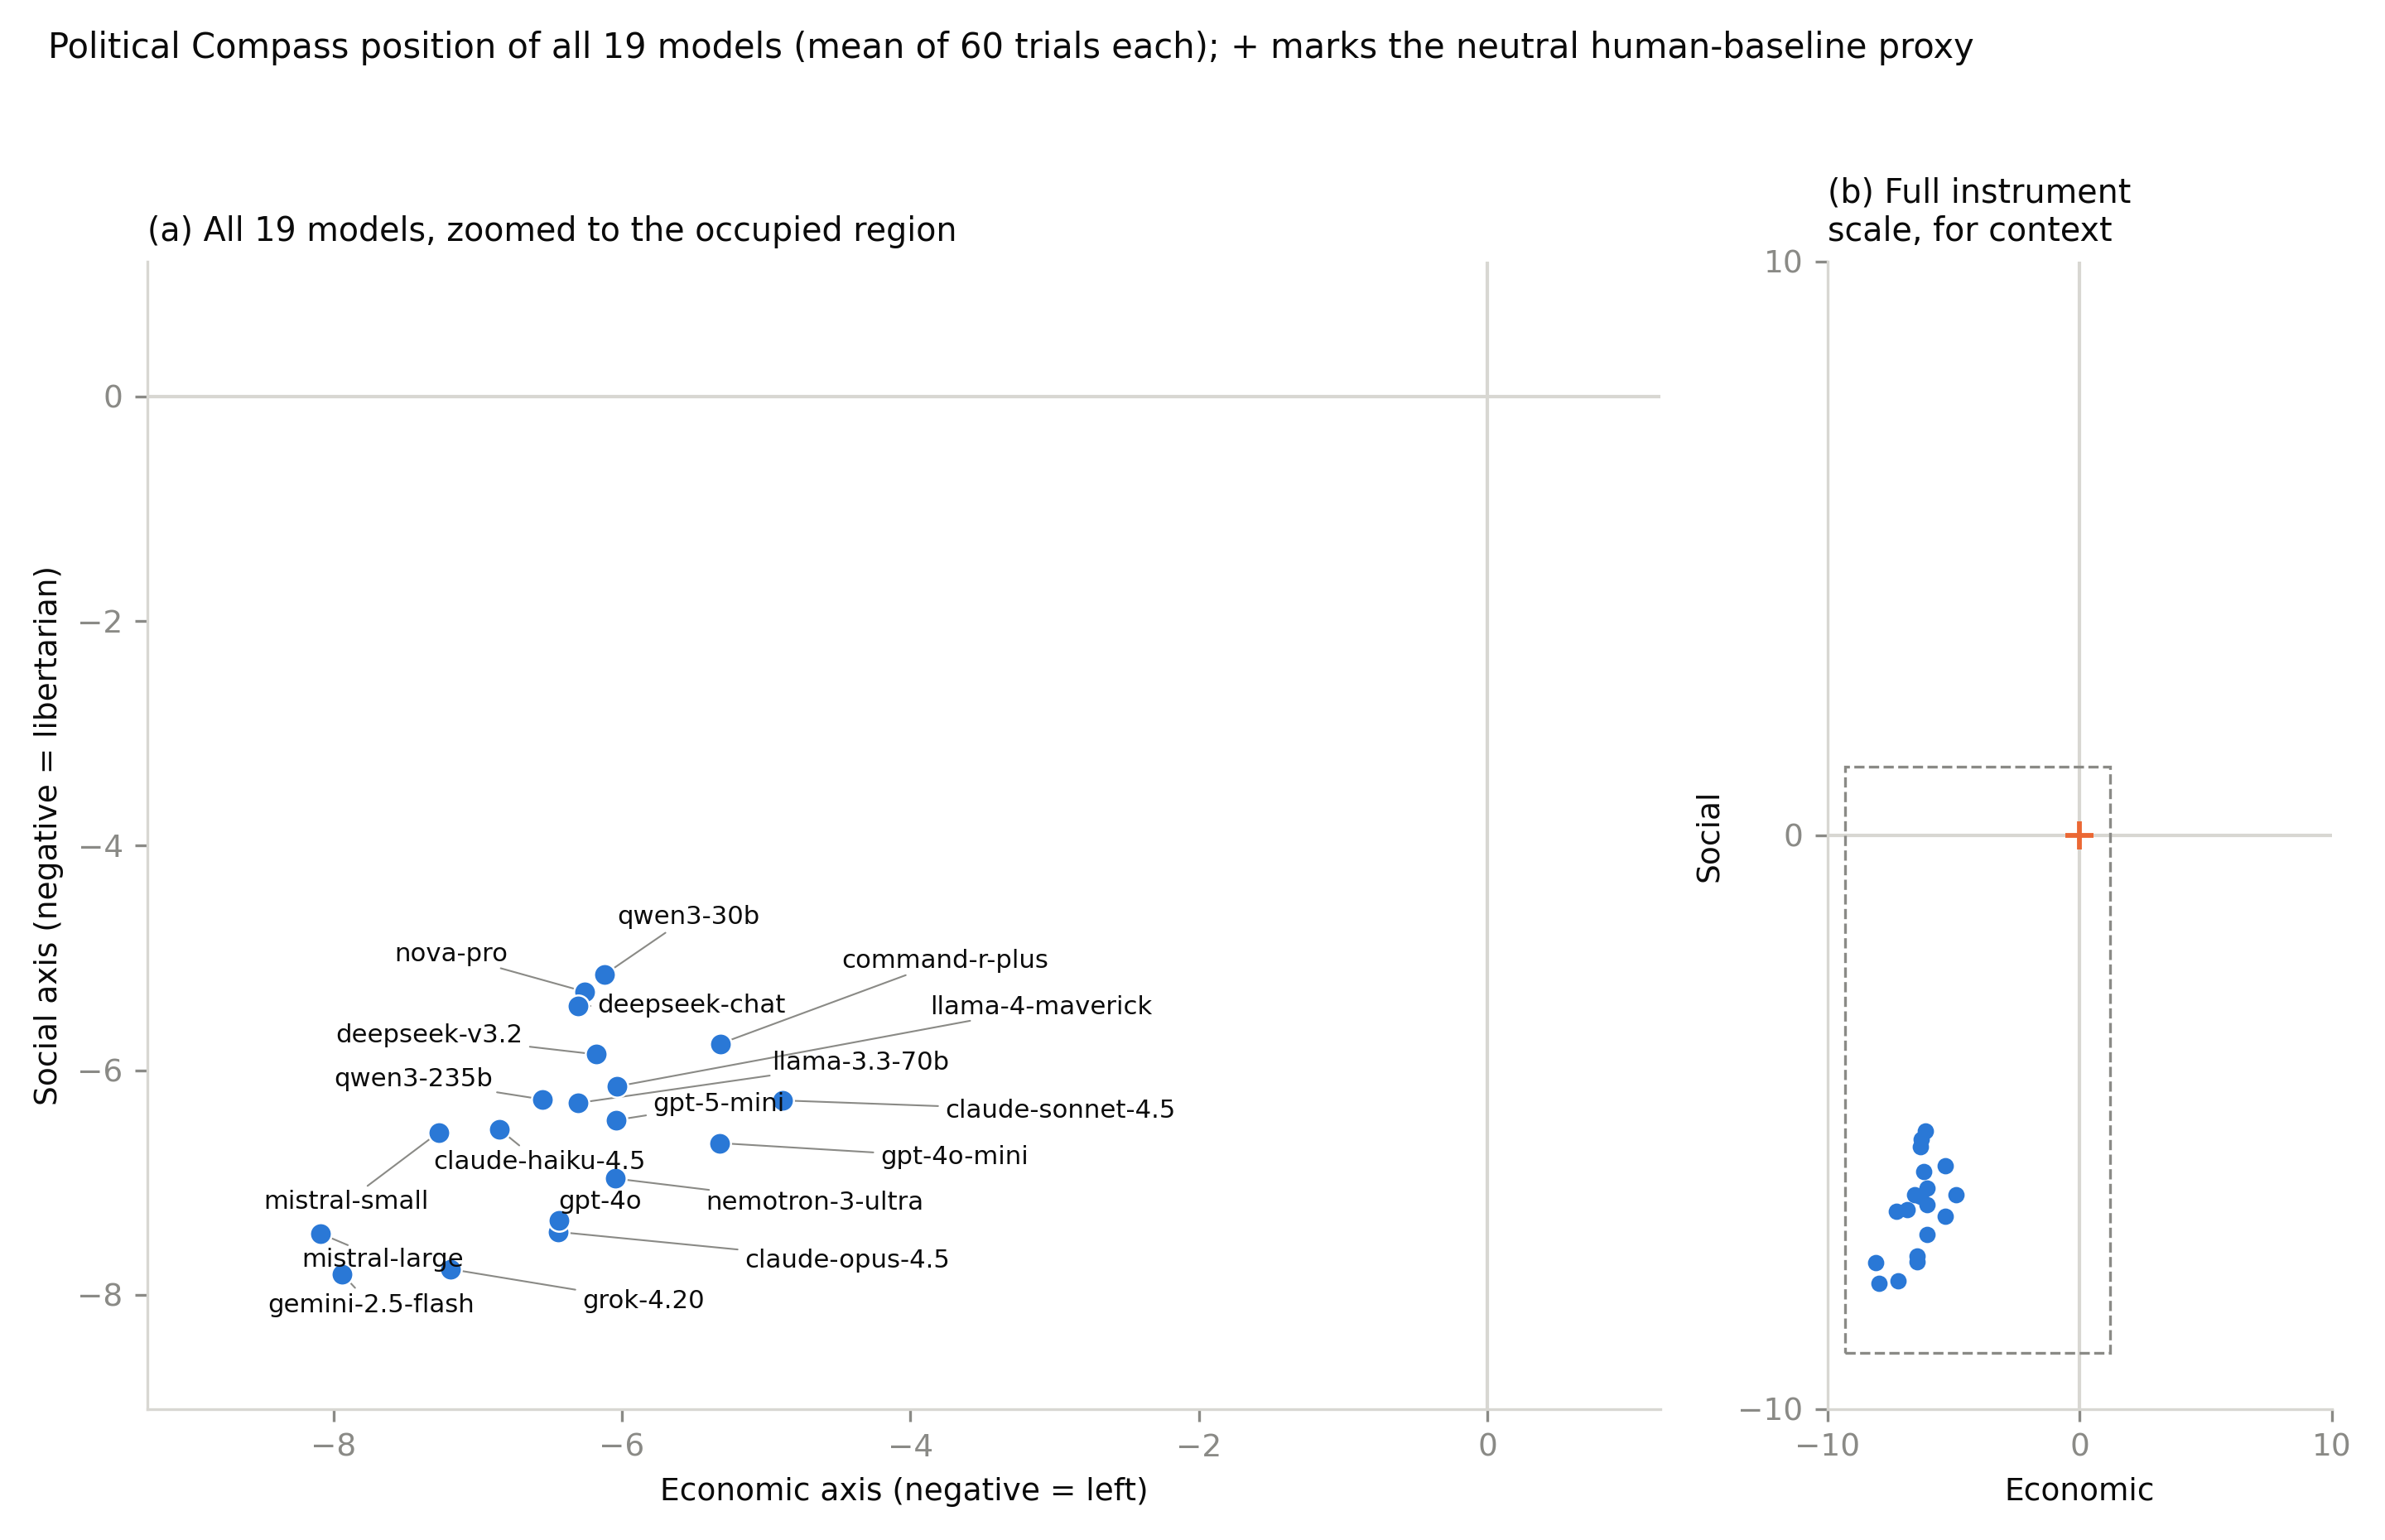
\includegraphics[width=0.95\textwidth]{figures/fig3_compass_scatter.png}
\caption{Political Compass position of all 19 models (mean of 60 trials
each). All models fall in the economically left, socially libertarian
quadrant.}
\label{sfig:compass-scatter}
\end{figure}

\begin{figure}[H]
\centering
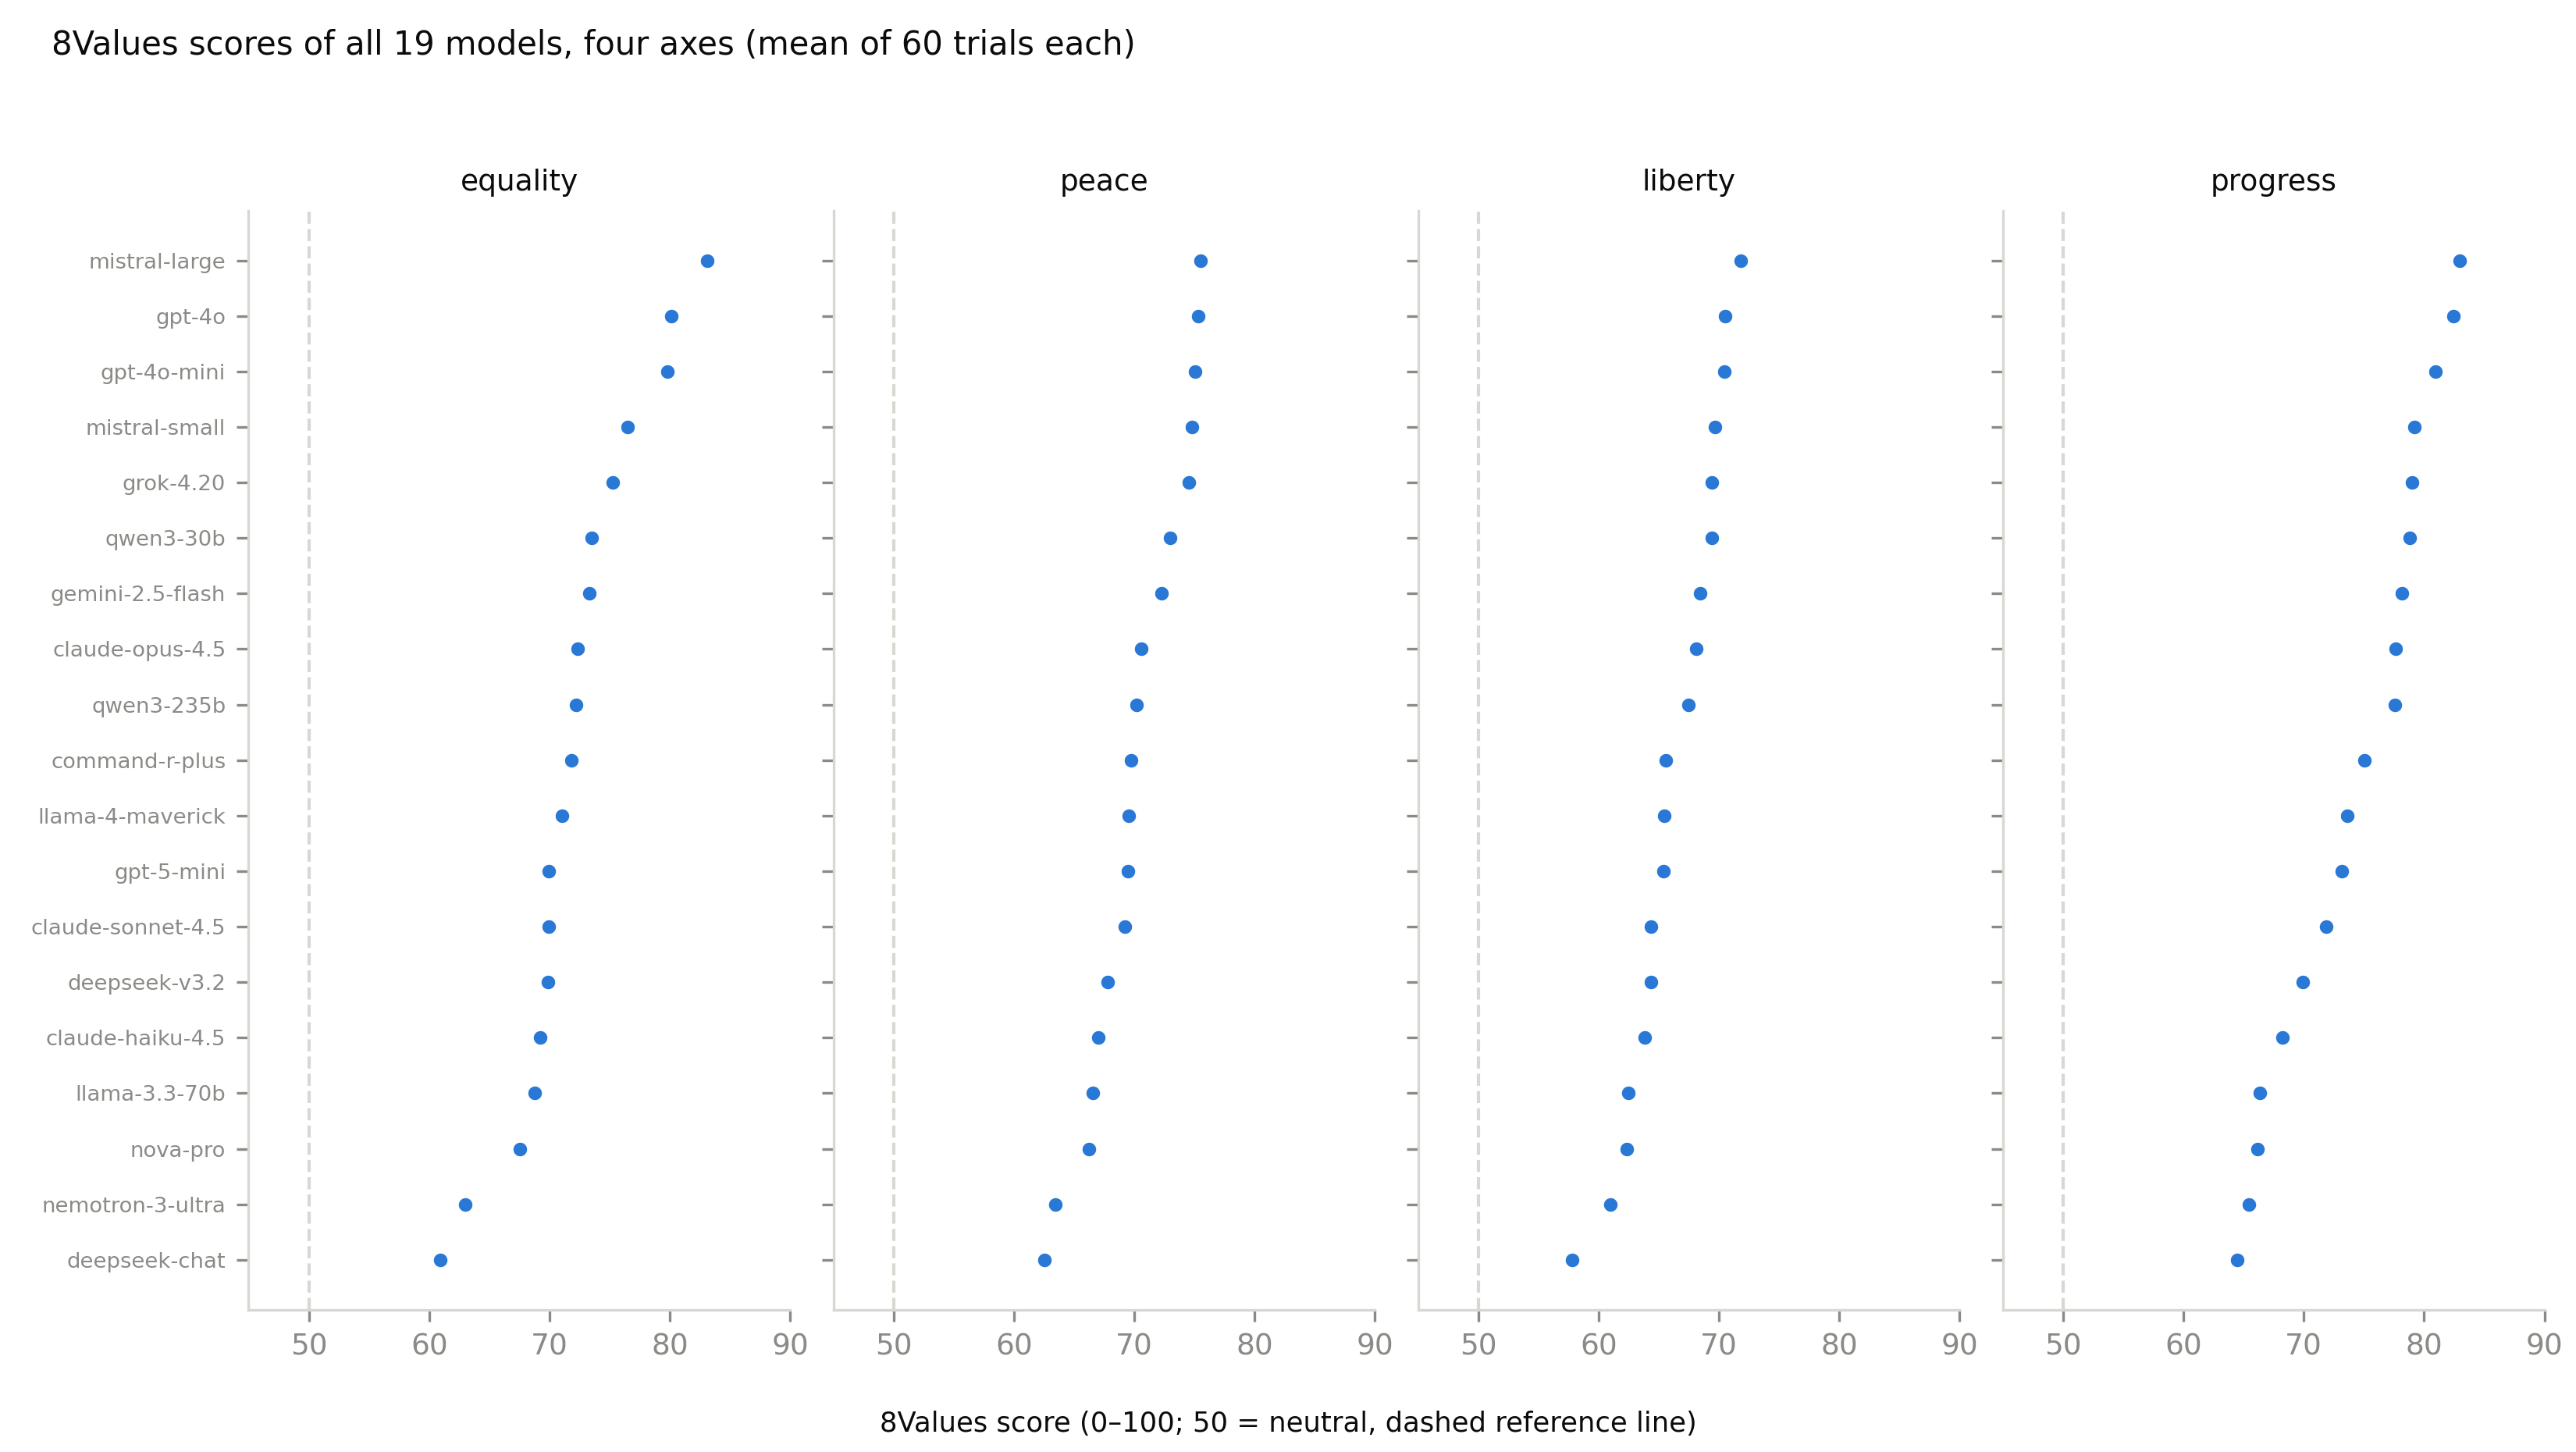
\includegraphics[width=\textwidth]{figures/fig4_8values_dotplot.png}
\caption{8Values scores of all 19 models on all four axes (mean of 60 trials
each), sorted independently within each panel; the dashed line marks the
instrument's neutral center-point (50).}
\label{sfig:8values-dotplot}
\end{figure}

\section{Omnibus Tests: Large, Robust Effects on Every Axis}
\label{si:omnibus}

Table~\ref{stab:omnibus} reports the classical one-way ANOVA, Welch's ANOVA,
and the Kruskal-Wallis test, together with the omnibus eta-squared effect
size, for each of the six scored axes. All three tests agree at $p < .0001$
on every axis, and every effect size is large ($\eta^2$ between $0.5625$ and
$0.7263$). Shapiro-Wilk rejects normality for a majority of the 19 groups on
most axes (11 to 17 of 19 groups non-normal, depending on axis), and
Levene's test rejects equal variance on every axis ($p<.0001$ throughout),
which is why Welch's ANOVA and Kruskal-Wallis, not the classical ANOVA, are
treated as the primary evidence for these omnibus effects.

\begin{table}[H]
\centering
\caption{Omnibus tests across all 19 models, by axis. All three tests agree at every axis.}
\label{stab:omnibus}
\footnotesize
\begin{tabular}{llrrrr}
\toprule
Test & Axis & Classical $F$ & Welch $F$ & Kruskal-Wallis $H$ & $\eta^2$ \\
\midrule
8Values & Equality & 138.3 & 534.8  & 792.0 & 0.6896 \\
8Values & Peace    & 80.1  & 421.5  & 759.4 & 0.5625 \\
8Values & Liberty  & 89.3  & 459.2  & 753.5 & 0.5891 \\
8Values & Progress & 165.3 & 618.5  & 886.8 & 0.7263 \\
Pol.\ Compass & Economic & 124.8 & 2240.3 & 762.0 & 0.6670 \\
Pol.\ Compass & Social   & 163.3 & 1370.3 & 867.5 & 0.7239 \\
\bottomrule
\end{tabular}
\vspace{0.3em}

\footnotesize
\textit{Note:} all $p < .0001$ for all three tests, on every axis.
\end{table}

\section{Post-hoc Comparisons: Games-Howell as the Primary Test, Corrected for the Full Test Family}

With 19 groups, each axis has 171 pairwise comparisons, and six axes give a
full family of 1{,}026 pairwise tests reported across this paper. Because
equal variances are rejected on every axis, Games-Howell is treated as
primary, with Tukey HSD reported alongside. At raw $p<0.05$, Games-Howell
finds between 121 and 144 of the 171 pairs significant per axis (equality:
142; peace: 136; liberty: 131; progress: 144; economic: 121; social: 138),
812 of the 1{,}026 pairwise tests in total. Applying a Benjamini-Hochberg
false discovery rate correction across the full family of 1{,}026 tests,
rather than within each axis separately, leaves 809 of the 812 significant,
a negligible change (equality: 142/142; peace: 136/136; liberty: 131/131;
progress: 142/144; economic: 120/121; social: 138/138): the between-model
differences reported here are not an artifact of running many uncorrected
tests. The two post-hoc tests mostly agree with each other as well: wherever
Tukey finds a different result than raw-$p$ Games-Howell, only 5 to 9 pairs
per axis are significant under Tukey but not under Games-Howell, an
artifact of Tukey's equal-variance assumption rather than a real
disagreement about the larger pattern.

Several pairwise Games-Howell effect sizes (Hedges' $g$) on this dataset are
very large in magnitude, considerably larger than is typical for behavioral
data. This is not evidence of unusually large real differences so much as a
consequence of some models, particularly several Claude variants, having
extremely low within-model variance on some axes (Section~\ref{si:consistency}):
dividing a modest mean difference by a very small pooled standard deviation
produces a large standardized effect size even when the raw difference, on
each instrument's own $-10$-to-$10$ or 0-to-100 scale, is unremarkable.
Readers should interpret the reported Hedges' $g$ values alongside the raw
mean differences in Table~\ref{stab:descriptive}, not in isolation.

\section{Consistency: Range-Normalized Stability Varies by Model, not by Provider}
\label{si:consistency}

Ranking every model-axis combination by ISS (Section~\ref{si:stats}) shows
that the most and least consistent entries in the dataset are not
concentrated in any one provider, country, or size tier. Table
\ref{stab:iss-extremes} lists the ten most and ten least consistent
combinations out of all 114 (19 models $\times$ 6 axes).

\begin{table}[H]
\centering
\caption{Ten most and ten least consistent model-axis combinations by Ideological Stability Score (ISS). Lower ISS = more consistent.}
\label{stab:iss-extremes}
\footnotesize
\begin{tabular}{lr}
\toprule
Model (test/axis) & ISS \\
\midrule
\multicolumn{2}{l}{\textit{Most consistent}} \\
anthropic/claude-opus-4.5 (Pol.\ Compass/social) & 0.00 \\
anthropic/claude-opus-4.5 (8Values/peace)        & 7.62 \\
anthropic/claude-opus-4.5 (8Values/equality)     & 7.87 \\
anthropic/claude-sonnet-4.5 (Pol.\ Compass/social) & 8.26 \\
meta-llama/llama-3.3-70b (8Values/equality)      & 8.33 \\
anthropic/claude-sonnet-4.5 (Pol.\ Compass/economic) & 9.04 \\
amazon/nova-pro-v1 (Pol.\ Compass/economic)      & 9.21 \\
x-ai/grok-4.20 (8Values/peace)                    & 10.20 \\
meta-llama/llama-3.3-70b (8Values/peace)          & 12.11 \\
meta-llama/llama-3.3-70b (8Values/progress)       & 12.92 \\
\addlinespace
\multicolumn{2}{l}{\textit{Least consistent}} \\
qwen/qwen3-235b (8Values/equality)               & 34.14 \\
nvidia/nemotron-3-ultra (8Values/liberty)         & 35.58 \\
meta-llama/llama-4-maverick (8Values/liberty)     & 36.19 \\
deepseek/deepseek-chat (8Values/equality)         & 37.45 \\
google/gemini-2.5-flash (8Values/peace)           & 37.71 \\
nvidia/nemotron-3-ultra (8Values/peace)           & 40.50 \\
nvidia/nemotron-3-ultra (8Values/progress)        & 41.39 \\
nvidia/nemotron-3-ultra (8Values/equality)        & 42.76 \\
anthropic/claude-haiku-4.5 (Pol.\ Compass/economic) & 44.42 \\
anthropic/claude-opus-4.5 (Pol.\ Compass/economic) & 65.22 \\
\bottomrule
\end{tabular}
\end{table}

Table~\ref{stab:iss-extremes} shows only the twenty most extreme entries;
Figure~\ref{sfig:iss-distribution} shows the full distribution of all 114
ISS values, grouped by axis, and makes visible both the general spread
within each axis and the single high-leverage outlier
(anthropic/claude-opus-4.5's Political Compass economic score) discussed
below.

\begin{figure}[H]
\centering
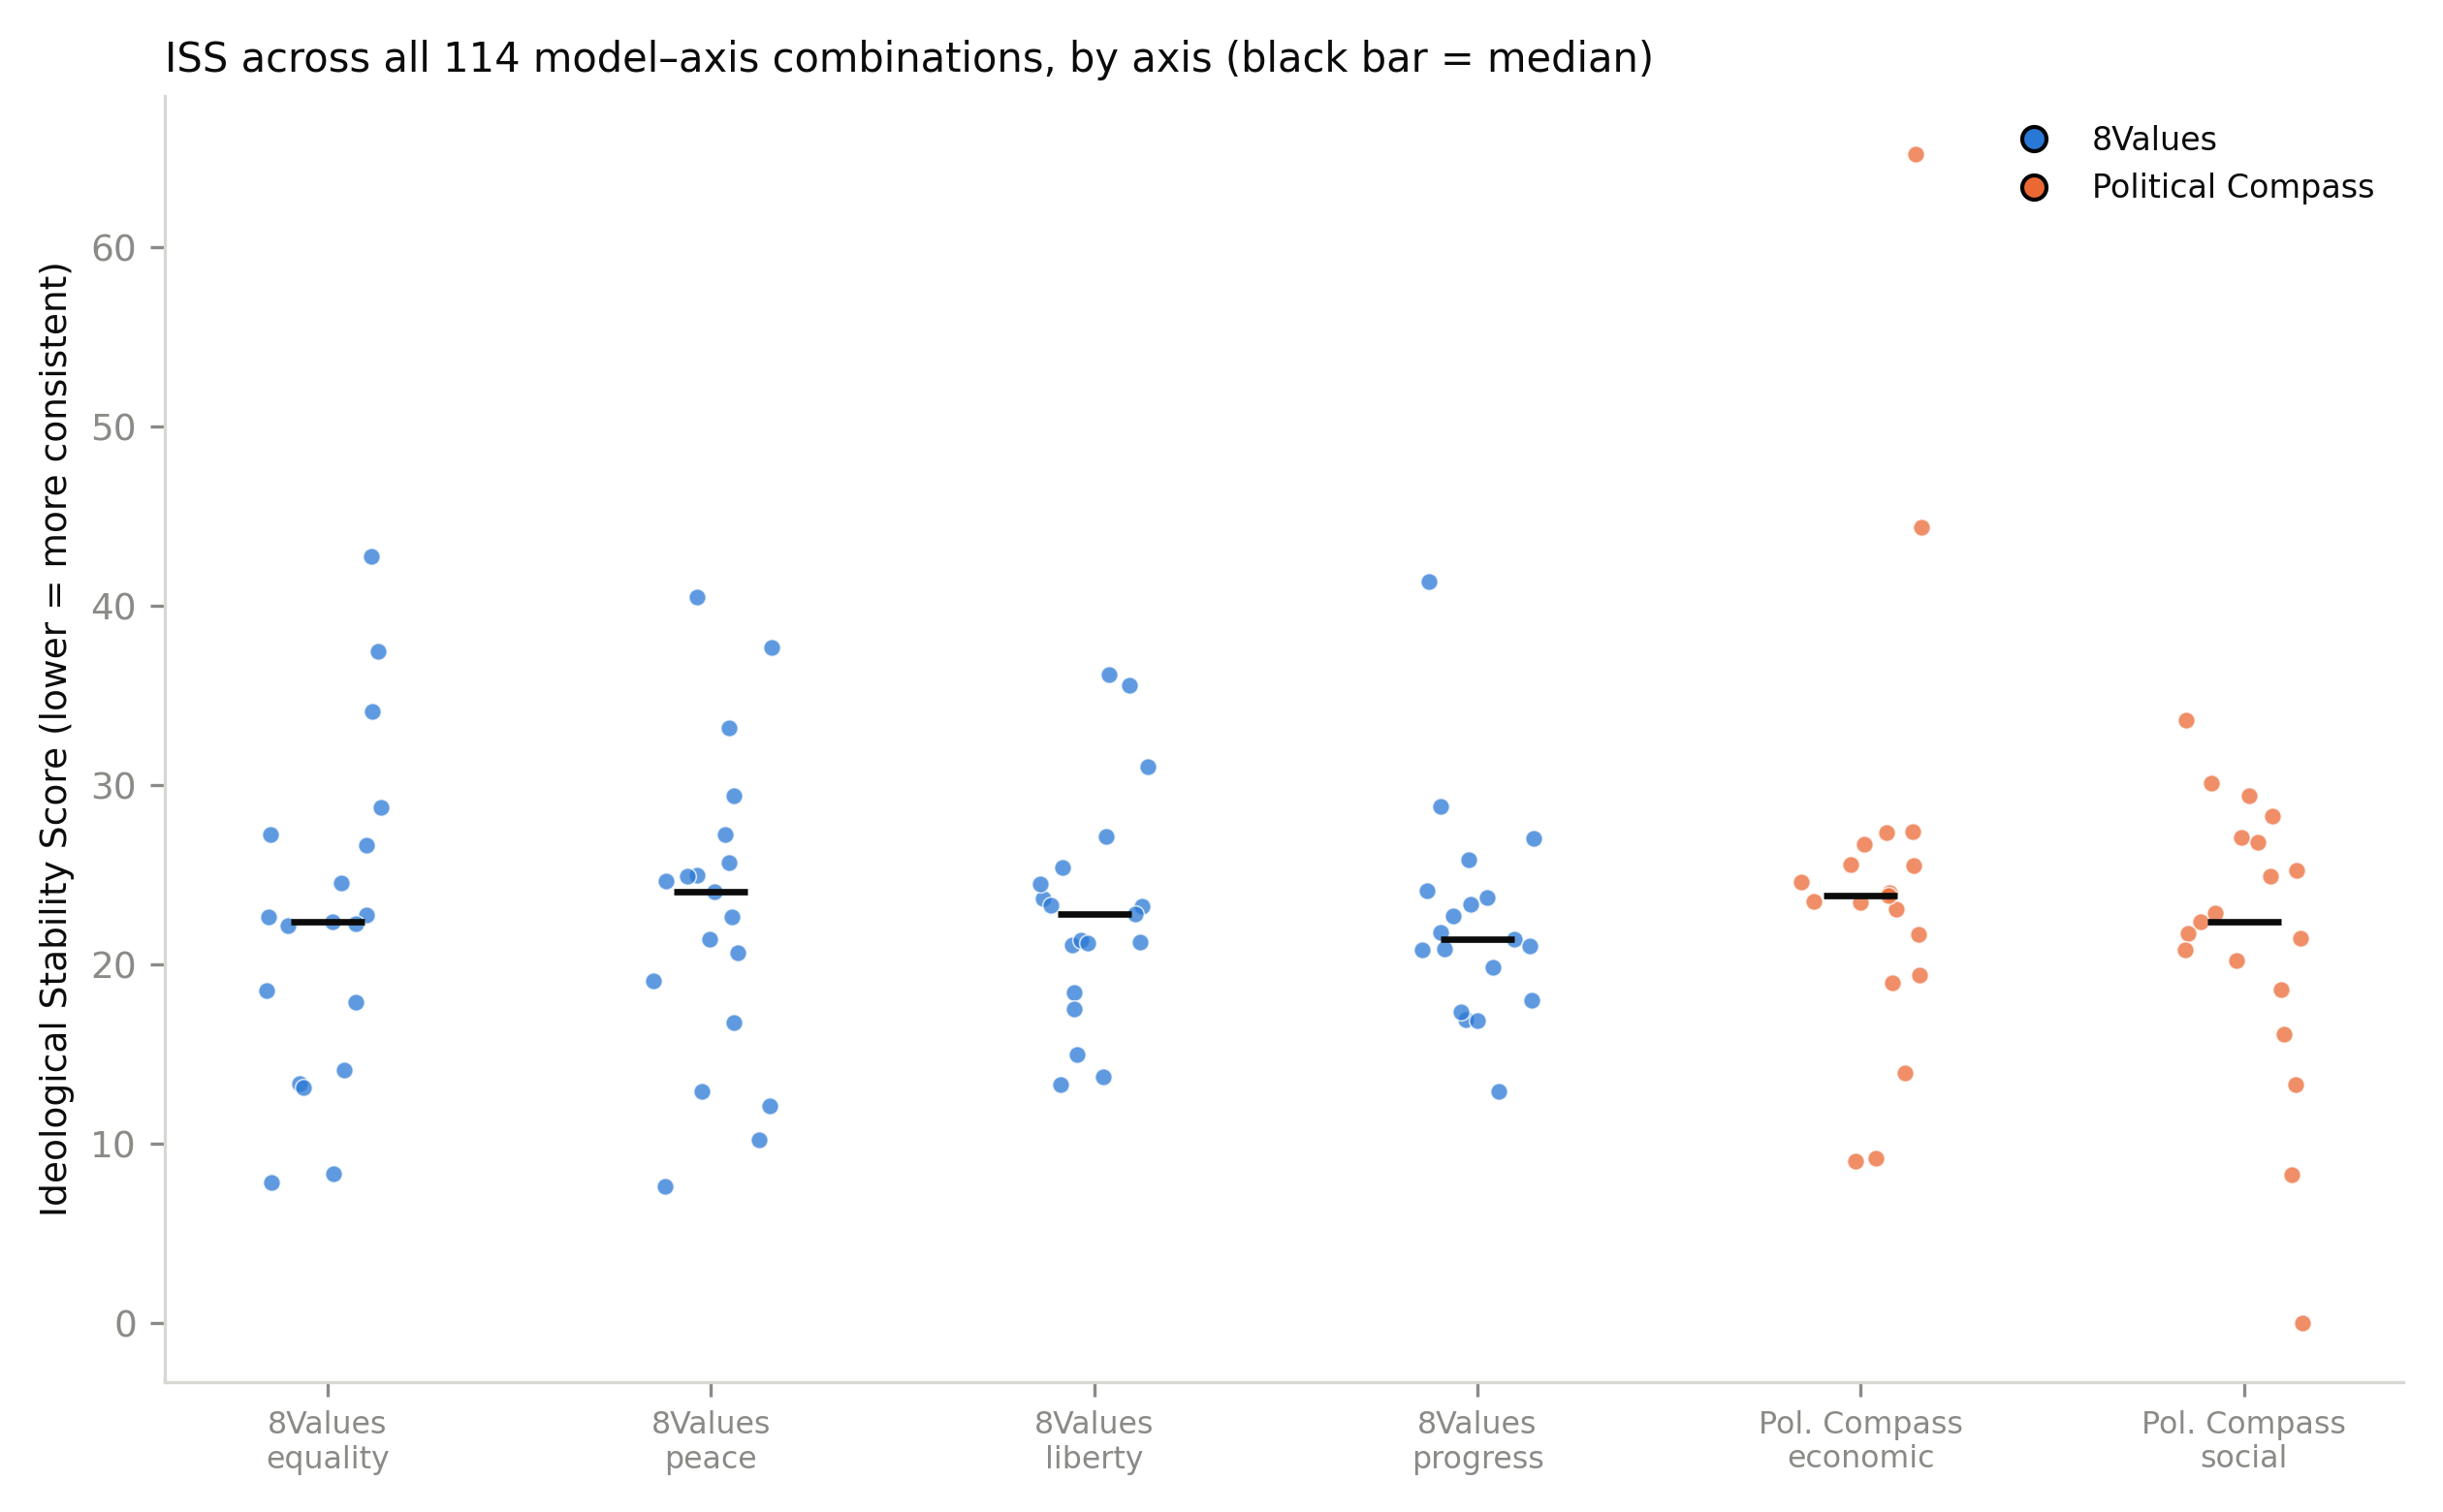
\includegraphics[width=0.85\textwidth]{figures/fig5_iss_distribution.png}
\caption{Ideological Stability Score for all 114 model--axis combinations,
grouped by axis. Each point is one model; the black bar marks the axis
median.}
\label{sfig:iss-distribution}
\end{figure}

anthropic/claude-opus-4.5 and meta-llama/llama-3.3-70b-instruct each appear
three times among the ten most consistent combinations, more than any other
model, while nvidia/nemotron-3-ultra-550b-a55b appears four times among the
ten least consistent. No provider is exclusively at either extreme: Claude
variants appear among both the single most consistent entry and, on a
different axis, the single least consistent entry in the entire dataset.

That last case illustrates the ISS range-normalization caveat from
Section~\ref{si:stats} directly, and is the reason the Letter reports
dispersion in the instrument's own units and the residual variance
component of the error budget instead of ISS. The Political Compass
economic score of anthropic/claude-opus-4.5 across its 60 trials took only
two distinct values, $-6.50$ and $-6.38$, an absolute range of $0.12$ on a
$-10$-to-$10$ scale; normalizing by that tiny self-range produces the
highest ISS in the dataset ($65.22$) despite the underlying answers being,
in absolute terms, essentially constant. By contrast, the same model's
Political Compass social score was literally identical across all 60 trials
($-7.44$ every time, ISS $= 0.00$). Both figures describe a model giving
highly stable absolute answers; the ISS score for the economic axis should
be read as an artifact of the metric's normalization, not as evidence of
erratic behavior. anthropic/claude-haiku-4.5's economic-axis ISS ($44.42$)
reflects a genuinely larger absolute range ($-7.38$ to $-6.38$) and is a
more straightforward instance of comparatively lower consistency. Across
all 114 model--axis cells, ISS correlates with absolute dispersion (standard
deviation) at only $\rho = 0.47$
(Figure~\ref{sfig:iss-repair}), which is the quantitative version of the
same point: ISS is not, in general, a good proxy for how much a model's
answers actually vary.

\begin{figure}[H]
\centering
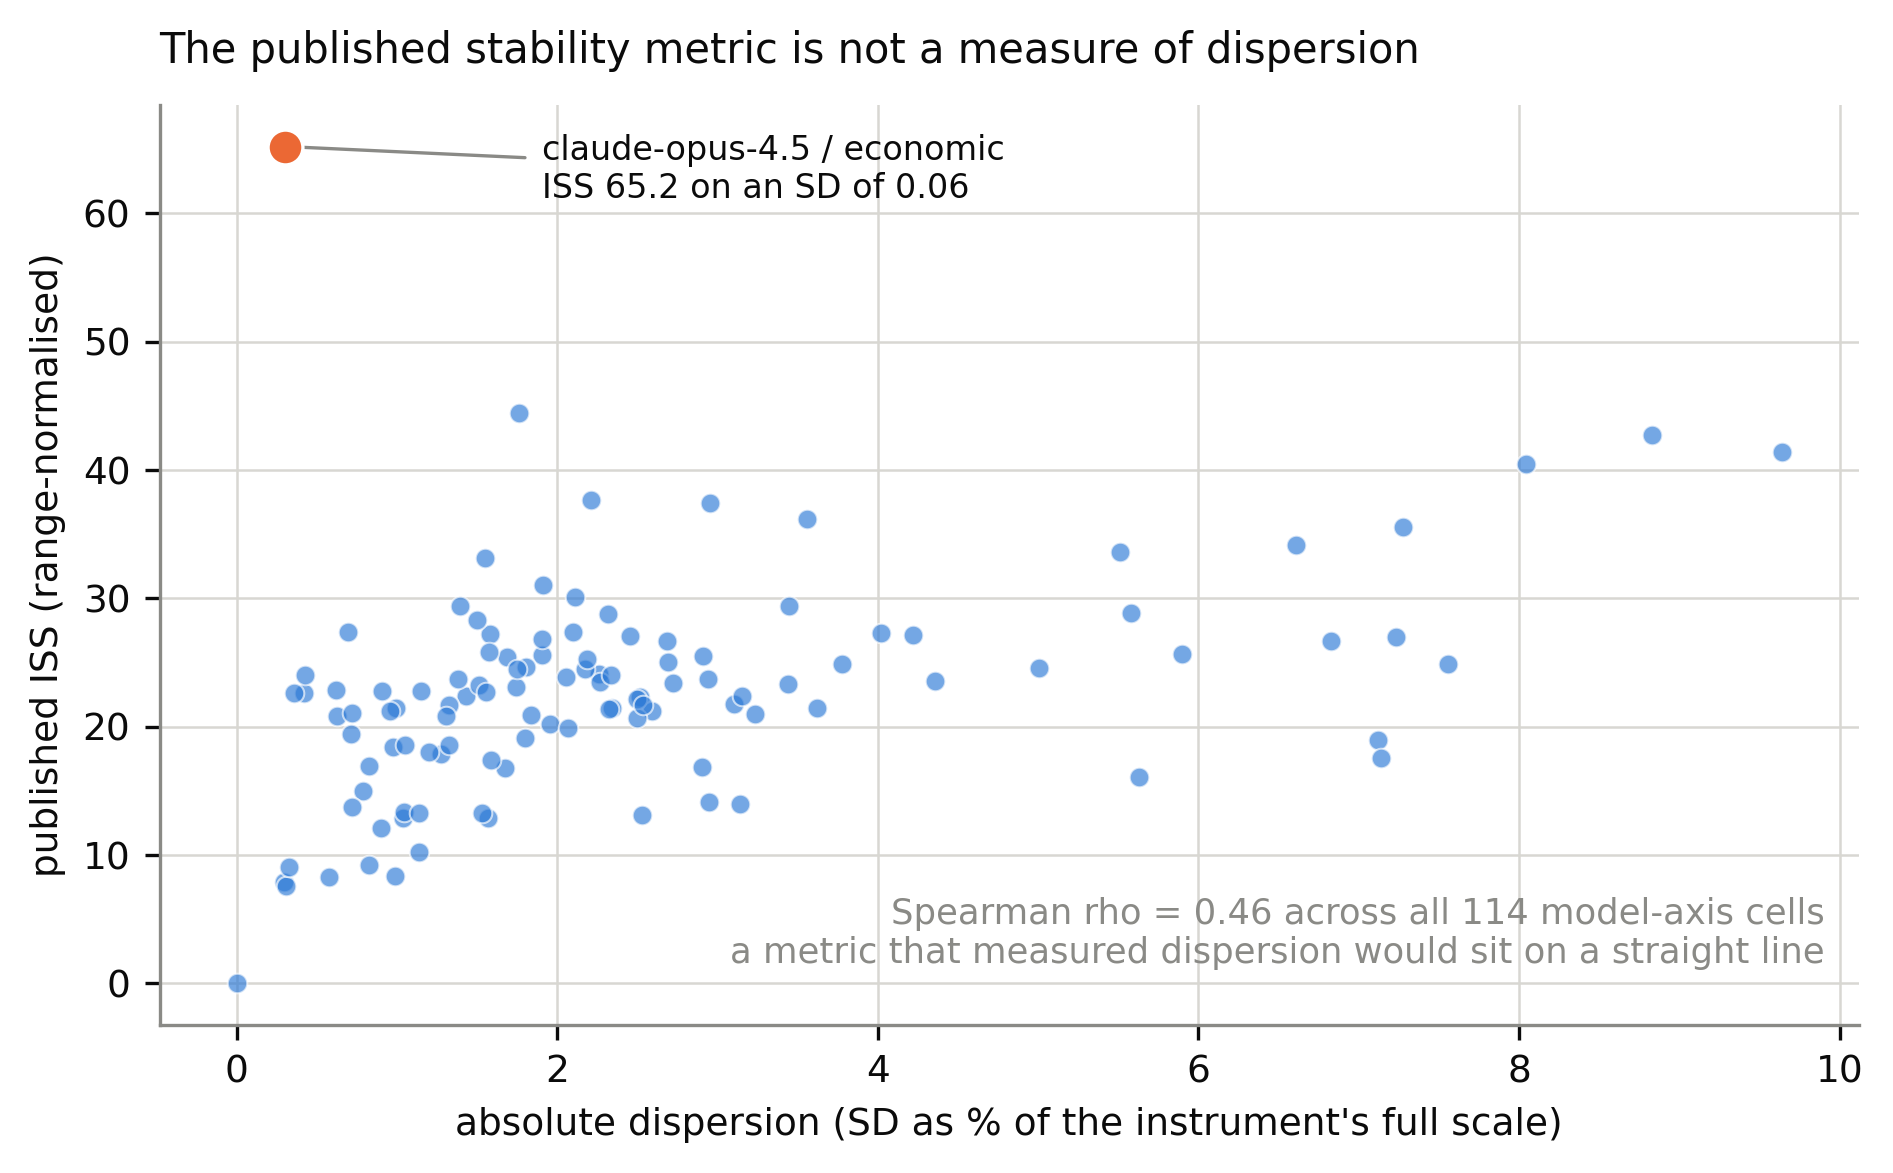
\includegraphics[width=0.78\textwidth]{figures/fig7_iss_repair.png}
\caption{The range-normalised stability metric is not a measure of
dispersion. Each point is one model--axis cell. Normalising by each
sample's own observed range inflates the score for models whose answers are
tightly clustered: the highlighted cell registers 65.2 on a standard
deviation of 0.060. Across all 114 cells the metric correlates with
absolute dispersion at only $\rho=0.47$.}
\label{sfig:iss-repair}
\end{figure}

\section{Comparison Against a Human-Population Reference Point}
\label{si:human-baseline}

Beyond comparing models to each other, every one of the 114 model-axis
combinations (19 models $\times$ 6 axes) differs significantly from that
instrument's own neutral center-point (one-sample $t$-test against 0 for the
two Political Compass axes and against 50 for the four 8Values axes), and
this holds for all 114 tests even after a Benjamini-Hochberg false discovery
rate correction. Given that Gallup's 2024 Values and Beliefs poll finds the
US public close to an even three-way split between conservative, moderate,
and liberal self-identification on social issues, and only moderately
right-of-center on economic issues \citep{gallup2024values}, a neutral
center-point is a reasonable, if bounded, proxy for a human population
reference (Section~\ref{si:stats}). Every model in this study, without
exception, differs significantly from that proxy, in the same direction
identified in the between-model comparisons above: left of center
economically and libertarian of center socially.

Statistical significance alone is a weak claim at $n=60$ trials per test,
since even a small, practically unremarkable deviation from center would
clear $p<0.05$ at that sample size. The effect sizes rule this out:
computing a one-sample Cohen's $d$ for each of the 114 tests (the
standardized deviation of a model's mean from the instrument's
center-point) finds every finite value at $|d|\geq 1.47$, comfortably past
Cohen's conventional threshold for a ``large'' effect ($|d|\geq 0.8$)
\citep{cohen1988}, with a median $|d|$ of $11.92$ and a maximum of $106.74$
(one model-axis combination is excluded from these summary statistics for
having an effectively zero within-model standard deviation, discussed in
Section~\ref{si:consistency}). The deviation from the neutral center-point
is therefore not merely statistically detectable but, on average, an order
of magnitude larger than the conventional threshold for a large effect.

\section{Prompt-Robustness Check: Magnitude Shifts, Direction Does Not}
\label{si:prompt-robustness}

Across the five-model, four-variant check (Section~\ref{si:robustness-checks}),
prompt wording produced a statistically significant shift in 29 of 30
model-axis combinations tested (one-way ANOVA across the five prompt
conditions, $p<0.05$), and the effect size was large ($\eta^2 \geq 0.14$) in
28 of those 30, with $\eta^2$ ranging from 0.02 to 0.75 (median 0.37). This
is a genuine, non-trivial finding, not a null result: instructional-wrapper
wording measurably moves scores for most models on most axes, consistent
with Röttger et al.'s critique that forced-choice political-typology
evaluations are sensitive to exactly how the task is framed
\citep{rottger2024}.

What did not move is direction. Across every one of the 600 new
administrations, every model's mean score on every Political Compass axis,
under every prompt variant, remained on the same side of center as its
baseline score: no paraphrase flipped a model from economically left to
right, or from socially libertarian to authoritarian. The largest single
shift observed was \texttt{openai/gpt-4o-mini}'s 8Values equality score,
ranging from 74.09 to 85.70 (an 11.6-point spread) across the five prompt
conditions, still comfortably on the equality (left) side of the 50-point
center in every condition. The directional finding that every model leans
the same way on every axis is therefore robust to prompt wording; the exact
magnitude of that lean, and consequently any fine-grained ranking between
closely-scored models, should be treated as sensitive to the specific
wording used and not over-interpreted.

\section{Open-Ended-Generation Validation Arm}
\label{si:openended-results}

Across the 120 judged generations (Section~\ref{si:robustness-checks}), the
correlation between a model's mean Political Compass score and its mean
judge-rated lean when writing open-endedly about matched-axis topics was
weak and not statistically significant on either axis (economic Pearson
$r=-0.56$, $p=0.32$; social $r=0.27$, $p=0.67$; $n=5$ models). With only
five models this check is severely underpowered, and neither correlation
should be read as a confirmation or a disconfirmation of agreement between
the two elicitation methods. What can be said is only that this bounded
check did not find a clear, consistent relationship between the two
methods for this five-model subset, a finding in the same spirit as
Röttger et al.'s broader point that forced-choice and open-ended
elicitation can diverge \citep{rottger2024}, and one that argues for a
larger-scale version of this arm (more models, more topics) before drawing
a firm conclusion either way.

\section{Item-Response-Theory Reanalysis}
\label{si:irt}

The published Political Compass and 8Values scoring keys treat every item
as equally informative and cannot separate a model declining to engage from
a model holding a genuinely moderate position \citep{wachter2025irt}. We
refit a graded-response IRT model separately on each of the six axes (the
four 8Values axes and the two Political Compass axes), using every
item-level response in the baseline dataset (19 models $\times$ 60 trials),
and compare the resulting latent trait ($\theta$) against each model's
published axis score.

\textbf{The published scores track the IRT-derived positions closely on
five of the six axes.} Spearman correlations between $\theta$ and the
published score range from $\rho=0.86$ to $\rho=0.94$ ($p<10^{-5}$ in every
case) on 8Values equality, peace, liberty, and progress and on the
Political Compass social axis, with narrow Bland-Altman limits of agreement
(Table~\ref{stab:irt-summary}). \textbf{The exception is the Political
Compass economic axis}, where $\rho=0.64$ and the limits of agreement are
roughly twice as wide as on any other axis. That axis has only 11 items,
the fewest of the six, and half its information comes from just 2 of them
(Table~\ref{stab:irt-summary})---the published economic score for this
instrument rests on the fewest and least-distributed items in the study,
which is a specific, checkable reason to weight it less heavily than the
other five axes rather than a general indictment of the scoring approach.

\textbf{Information is concentrated in a minority of items on every axis.}
Between 4 and 12 items (out of 11 to 50 per axis) carry half of each axis's
total discrimination, and the top decile of items by discrimination
carries 24--33\% of it. A small, identifiable subset of items is doing most
of the work of separating models on every axis we fit, on both instruments.

\textbf{Neutral-response rates vary roughly five-fold across models on
8Values} (9\% to 52\% of items answered at the scale midpoint), which is the
avoidance behaviour \citet{wachter2025irt} predict: at least part of the
apparent centrism in the most avoidant models is a refusal to commit to
either pole rather than a moderate position, and it is not evenly
distributed across the cohort. We do not have a validated way to convert a
neutral-rate estimate into a bias correction for the published score, so we
report it as a per-model caveat rather than an adjustment.

\begin{table}[H]
\centering
\caption{IRT reanalysis summary by axis. $\rho$ is the Spearman correlation
between the IRT latent trait and the published axis score across the 19
models; LoA is the Bland-Altman 95\% limits of agreement, in the published
score's own units after within-axis standardization; ``items for half
info.'' is the minimum number of items whose summed discrimination reaches
half the axis total.}
\label{stab:irt-summary}
\footnotesize
\begin{tabular}{llrrrr}
\toprule
Instrument & Axis & Items & $\rho$ & LoA & Items for half info. \\
\midrule
8Values & Equality & 22 & 0.91 & $\pm 0.83$ & 4 \\
8Values & Peace & 24 & 0.86 & $\pm 0.88$ & 6 \\
8Values & Liberty & 37 & 0.92 & $\pm 0.61$ & 7 \\
8Values & Progress & 33 & 0.88 & $\pm 0.81$ & 7 \\
Political Compass & Economic & 11 & 0.64 & $\pm 1.27$ & 2 \\
Political Compass & Social & 50 & 0.94 & $\pm 0.63$ & 12 \\
\bottomrule
\end{tabular}
\end{table}

\section{Multi-Trait Multi-Method Matrix}
\label{si:mtmm}

Figure~\ref{sfig:mtmm} shows the full correlation matrix behind the
convergent-validity result reported in the Letter. Convergent coefficients
(same construct, different instrument) average $r=-0.26$; discriminant
coefficients (different construct, same instrument) average $r=+0.52$
(Table~\ref{stab:mtmm}). The four 8Values axes correlate with one another
at mean $r=0.71$, consistent with a single dominant general factor rather
than four separable traits.

\begin{figure}[H]
\centering
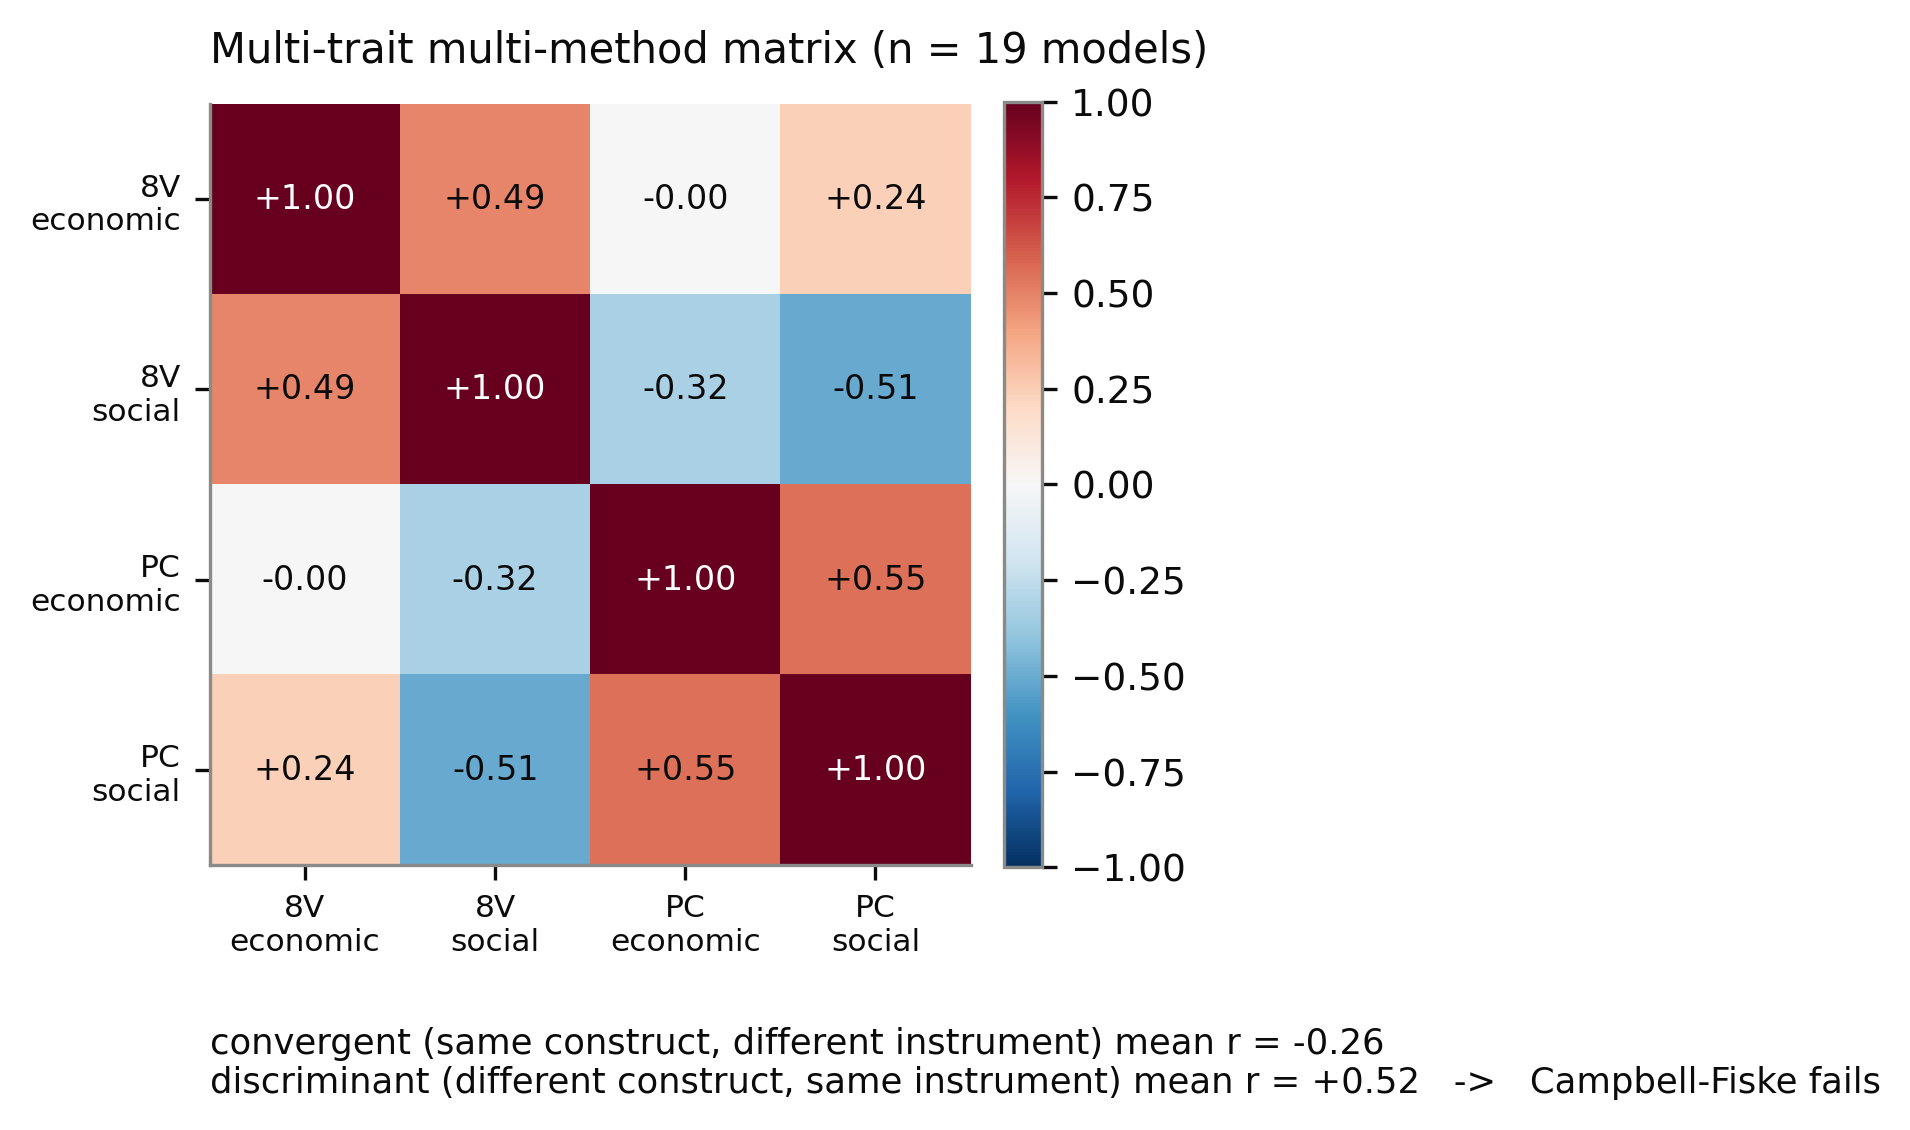
\includegraphics[width=0.72\textwidth]{figures/figSI_mtmm.png}
\caption{Multi-trait multi-method matrix across the 19 models. Convergent
coefficients (same construct, different instrument) average $r=-0.26$;
discriminant coefficients (different construct, same instrument) average
$r=+0.52$. The Campbell--Fiske ordering is inverted, so the two instruments
cannot be treated as interchangeable measures of a common political
position.}
\label{sfig:mtmm}
\end{figure}

\begin{table}[H]
\centering
\caption{Multi-trait multi-method coefficients across the 19 models. Convergent validity requires that the same construct measured by two instruments correlate more strongly than two different constructs measured by the same instrument. It does not.}
\label{stab:mtmm}
\begin{tabular}{llr}
\toprule
Type & Pair & $r$ \\
\midrule
Convergent & 8values:economic vs political\_compass:economic & -0.005 \\
Convergent & 8values:social vs political\_compass:social & -0.506 \\
Discriminant & 8values:economic vs 8values:social & +0.490 \\
Discriminant & political\_compass:economic vs political\_compass:social & +0.549 \\
\midrule
\textbf{Mean convergent} & & \textbf{-0.255} \\
\textbf{Mean discriminant} & & \textbf{+0.520} \\
\bottomrule
\end{tabular}
\end{table}

A preliminary check on a third instrument, SapplyValues, is consistent with
this picture rather than resolving it. The directional finding partly
replicates: all 18 models scored are economically left ($\text{right}<0$)
and culturally progressive ($\text{prog}>0$), matching the Political
Compass and 8Values baseline; the libertarian finding does not, with only 7
of 18 models scoring libertarian on SapplyValues' authority axis.
Correlating each SapplyValues axis against the existing axis that claims to
measure the same construct, across the 18 shared models, the economic axis
disagrees with Political Compass ($\rho=-0.49$, 95\% CI [$-0.78$, $-0.04$]
---bootstrap, negative where the shared ``positive means right'' convention
predicts positive) while agreeing with 8Values' equality axis in the
expected direction ($\rho=-0.53$, [$-0.87$, $-0.01$]). The authority-axis
comparisons are inconclusive at this sample size (95\% CIs spanning zero
against both other instruments). We read this as a third data point for the
same conclusion, not a resolution of it: adding an instrument did not
converge the disagreement onto a single answer, it added a third position.

A fourth instrument, Pew Research Center's 2026 Political Typology, gives
an authoritative check of a different kind (Section~\ref{si:remaining-factors-methods}):
rather than scoring an axis ourselves, we drove the live 24-item quiz with
each model's answers and read off the classification Pew's own site
computes, since Pew's clustering weights are not published. Sixteen of 18
models' modal classification falls left of centre (one of the four
left-leaning groups in Pew's own nine-group, left-to-right ordering);
two---\texttt{deepseek/deepseek-chat} and \texttt{x-ai/grok-4.20}---classify
as \emph{Pragmatic and Polite Right}, the first group right of centre, with
\texttt{x-ai/grok-4.20} landing there in all 10 of 10 trials. The ordinal
position of a model's classification (1--9, left to right) does not
correlate with its Political Compass economic score or 8Values equality
score across the 18 shared models ($\rho=0.04$, [$-0.39$, $0.51$], and
$\rho=-0.03$, [$-0.55$, $0.54$] respectively---both consistent with no
relationship at this sample size). The directional finding therefore
replicates on a fourth, independently classified instrument, with two clear
exceptions.

The four-instrument crossing reported in the Letter (model-identity share
1.89\%; SapplyValues alone, 0.49\%; Pew alone, 8.21\%) is the full
accounting that this section's pairwise checks anticipate. Between-model
spread and within-model trial noise are proportionally in line with the
other instruments for SapplyValues too (ratio $\approx 1.9$ for all three
continuous instruments), so the collapse is not a SapplyValues
data-quality artefact; it is what the objection ``a variance component
estimated from two instruments is meaningless'' looks like quantitatively
once a third and fourth instrument are added.

\section{Display Items Not Referenced Elsewhere}

\begin{figure}[H]
  \centering
  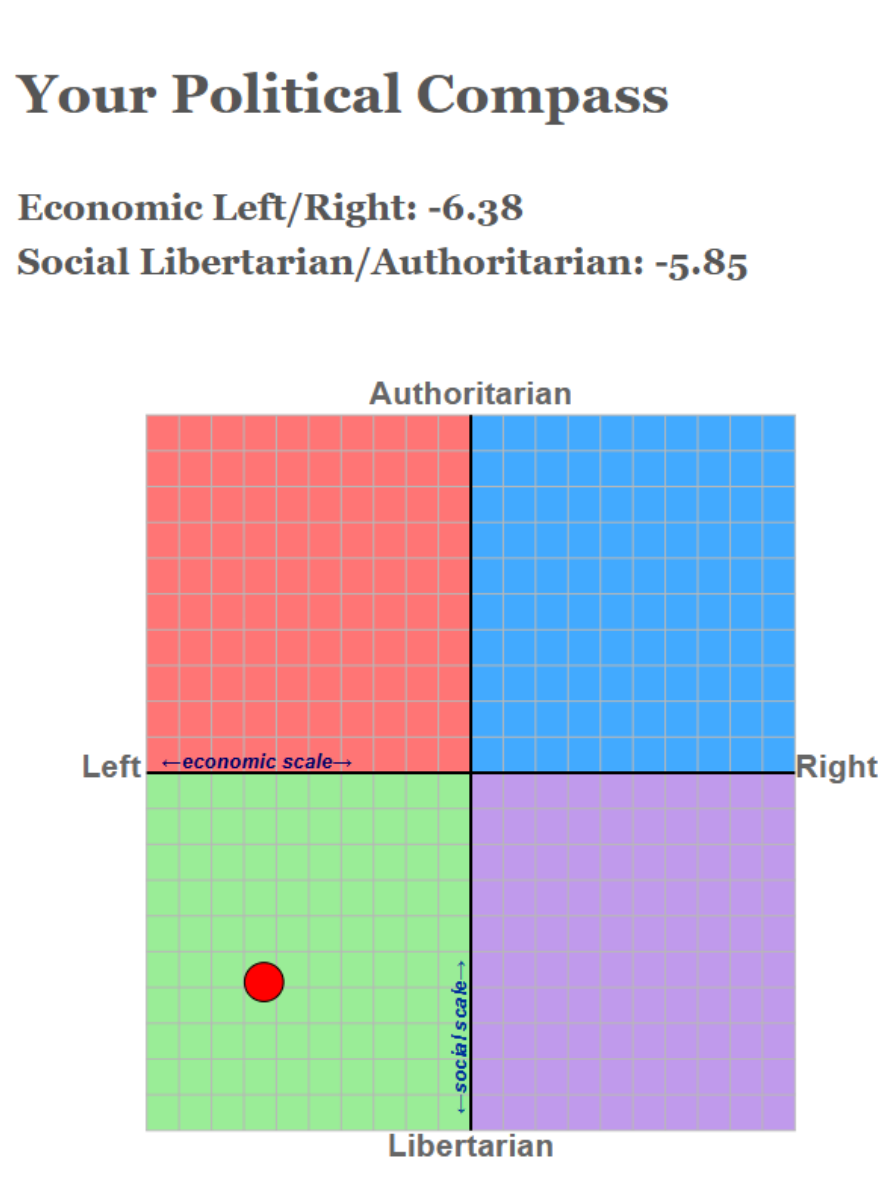
\includegraphics[width=0.55\textwidth]{figures/fig1_political_compass.png}
  \caption{Example Political Compass output for a single trial.}
  \label{sfig:polcompass}
\end{figure}
\begin{figure}[H]
  \centering
  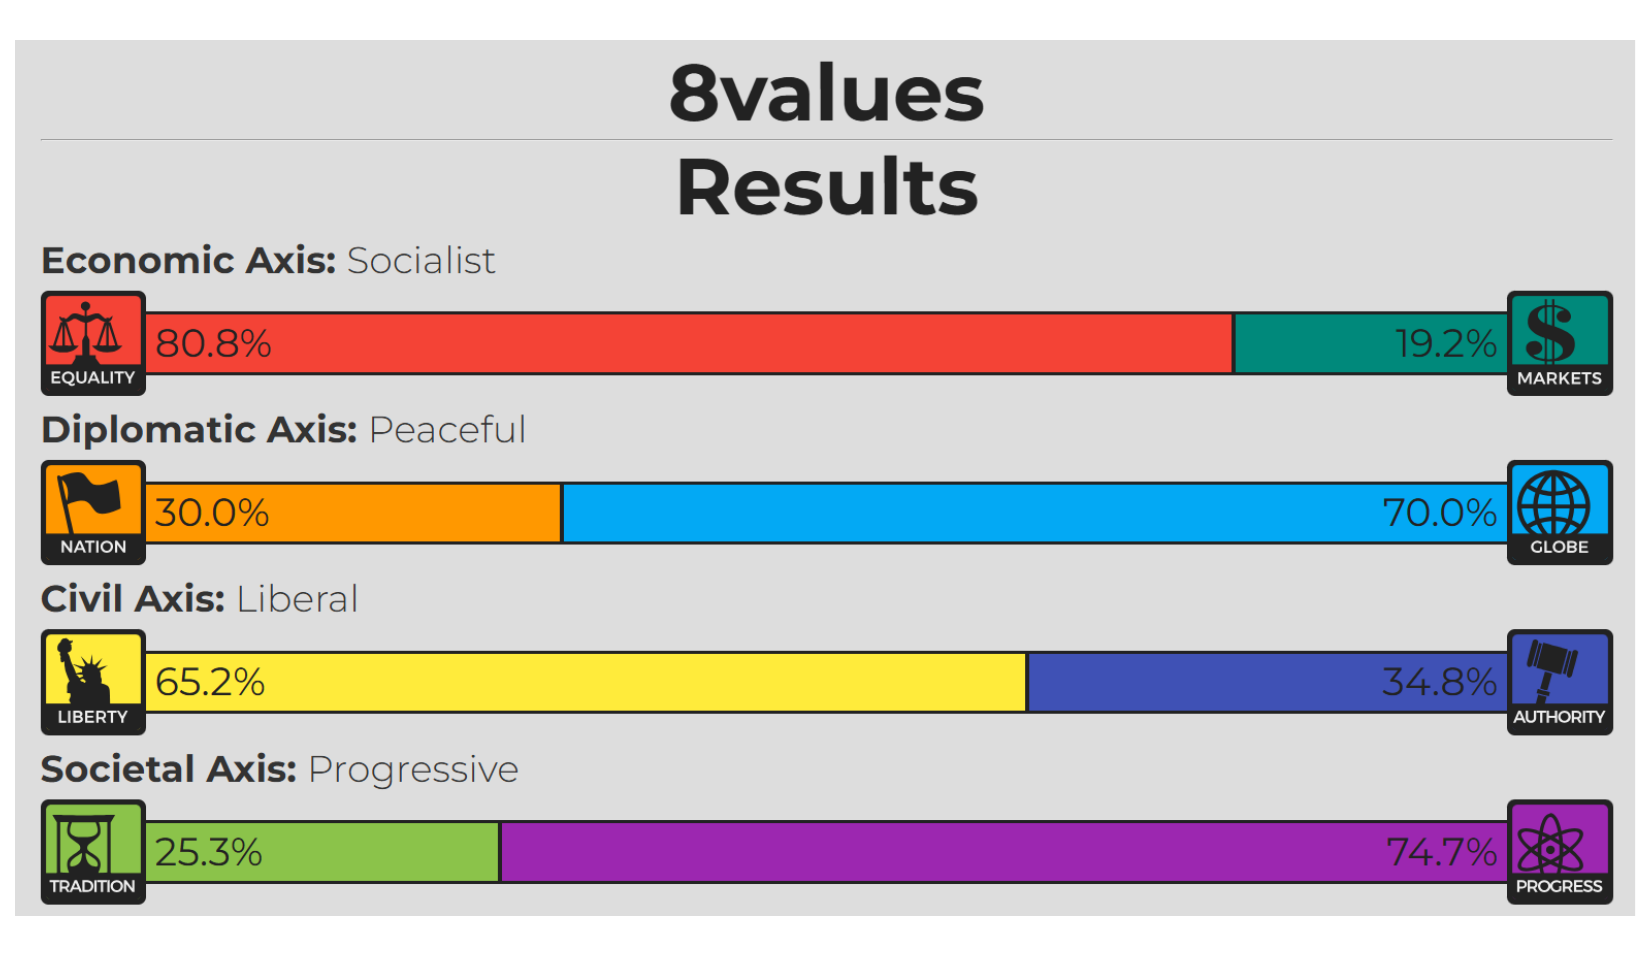
\includegraphics[width=0.85\textwidth]{figures/fig2_8values.png}
  \caption{Example 8Values output for a single trial.}
  \label{sfig:8values}
\end{figure}
\begin{table}[H]
\centering
\caption{Collection completion rate and cost by model (both tests combined, 120 administrations/model).}
\label{stab:collection-summary}
\footnotesize
\begin{tabular}{lrr}
\toprule
Model & Completion rate & Cost \\
\midrule
amazon/nova-pro-v1 & 100\% & \$0.31 \\
anthropic/claude-haiku-4.5 & 100\% & \$0.42 \\
anthropic/claude-opus-4.5 & 100\% & \$1.95 \\
anthropic/claude-sonnet-4.5 & 100\% & \$1.42 \\
cohere/command-r-plus-08-2024 & 100\% & \$0.98 \\
deepseek/deepseek-chat & 100\% & \$0.09 \\
deepseek/deepseek-v3.2 & 100\% & \$0.02 \\
google/gemini-2.5-flash & 100\% & \$0.21 \\
meta-llama/llama-3.3-70b-instruct & 100\% & \$0.04 \\
meta-llama/llama-4-maverick & 100\% & \$0.07 \\
mistralai/mistral-large-2512 & 100\% & \$0.11 \\
mistralai/mistral-small-3.2-24b-instruct & 100\% & \$0.02 \\
nvidia/nemotron-3-ultra-550b-a55b & 100\% & \$1.38 \\
openai/gpt-4o & 100\% & \$0.84 \\
openai/gpt-4o-mini & 100\% & \$0.04 \\
openai/gpt-5-mini & 100\% & \$0.59 \\
qwen/qwen3-235b-a22b & 100\% & \$0.49 \\
qwen/qwen3-30b-a3b & 100\% & \$0.14 \\
x-ai/grok-4.20 & 100\% & \$0.18 \\
\midrule
Total & 100\% (2{,}280/2{,}280) & \$9.30 \\
\bottomrule
\end{tabular}
\end{table}

\section{Data and Code Availability}
\label{si:availability}

All raw per-trial data from this study are released at a public repository
(link withheld from this appendix for anonymized review; provided to the
editor and restored on acceptance). This includes the main 2{,}280-administration
run across 19 models (\texttt{data/raw\_trials/}, with a flattened table in
\texttt{data/scores.csv} and a per-model completion-rate and cost summary in
\texttt{data/collection\_summary.md}); the 2{,}160-administration
asker-identity factorial and its 180-call probe (\texttt{data/asker\_identity/});
the 1{,}080-administration contamination factorial and its memorisation
probe (\texttt{data/item\_variants/}); the 4{,}320-administration
response-format factorial (\texttt{data/format\_factorial/}); a
540-administration baseline on a third instrument, SapplyValues (18
models, \texttt{data/raw\_trials/}, filenames containing
\texttt{sapplyvalues}); and a 180-administration baseline on a fourth
instrument, Pew's 2026 Political Typology (\texttt{data/pew\_typology/}).
Both the third and fourth instrument are crossed into the shared
variance-components model used for the first two
(\texttt{scoring/analyze\_f3\_variance\_components.py}; Section~\ref{si:remaining-factors-methods}).
Every record includes the model's structured JSON answers, the resulting
score, and the exact API cost of that call.

The complete pipeline, including the collection script, both scoring
adapters (the 8Values port and the Political Compass browser-automation
adapter), the consolidation script, the figure-generation script, and the
full statistical analysis script, is released as open source at the same
repository. No code is reproduced in the body of this paper; the repository
is the authoritative source for exact implementation details and is kept
in sync with the analyses reported here.

\section{Declarations}
\label{si:ethics}

\subsection*{Author Contributions}
The author conceived the study, designed and built the data-collection and
scoring pipeline, collected and statistically analyzed the data, and wrote
the manuscript.

\subsection*{Competing Interests}
The author declares no competing interests.

\subsection*{Funding}
[To be completed on the title page / submission system.]

\subsection*{Ethics Declarations}
This study did not involve human participants, human data, or animal
subjects. All data consist of text outputs generated by third-party large
language models accessed via a commercial API (OpenRouter); no personal,
sensitive, or identifiable information is involved. Institutional ethics
review was therefore not required.

One instrument, Pew Research Center's 2026 Political Typology (Section~\ref{si:remaining-factors-methods}),
was scored by programmatically driving Pew's live public quiz and reading
off its own classification, rather than reimplementing Pew's unpublished
clustering procedure, following the same approach already used for
Political Compass. Reusing the instrument's item text and published group
definitions for research is covered by Pew's general terms of use.
Submitting the interactive quiz itself 180 times in an automated fashion is
a distinct question: it plausibly exceeds ordinary personal use of that
interactive tool, even though it accesses no respondent microdata or
personal information at any point. We disclose this explicitly rather than
treating it as settled by the terms-of-use analysis for the survey items.

\bibliographystyle{chicago}
\bibliography{references}
\end{document}
